% =====================================================================
%  HALQA — Official Final Report, IEEE WIE ACT 5.0 / EdNova Challenge
%  IEEE WIE ACT 5.0 · EdNova GenAI Peer-Learning Companion Challenge
%  Compile: tectonic main.tex   (or pdflatex + bibtex-free, no external deps)
%  Grayscale, print-ready, A4, 11pt.
% =====================================================================
\documentclass[10pt,a4paper,oneside]{report}

\usepackage[utf8]{inputenc}
\usepackage[T1]{fontenc}
\usepackage{lmodern}
\usepackage[english]{babel}

\usepackage[a4paper,top=2.0cm,bottom=2.0cm,left=2.15cm,right=1.95cm,headsep=0.55cm,footskip=0.95cm]{geometry}

\usepackage{graphicx}
\usepackage{amsmath,amssymb}
\usepackage{booktabs}
\usepackage{longtable}
\usepackage{array}
\usepackage{tabularx}
\usepackage{enumitem}
\setlist[itemize]{leftmargin=1.15em,itemsep=1pt,topsep=2pt,parsep=0pt}
\setlist[enumerate]{leftmargin=1.35em,itemsep=1pt,topsep=2pt,parsep=0pt}
\setlist[description]{leftmargin=0pt,itemsep=1pt,topsep=2pt,parsep=0pt}
\usepackage{fancyhdr}
\usepackage{titlesec}
\usepackage{caption}
\usepackage{subcaption}
\usepackage[dvipsnames,table]{xcolor}
\usepackage{tikz}
\usetikzlibrary{arrows.meta,positioning,fit,backgrounds,calc,shapes.geometric,shadows.blur,decorations.pathreplacing}
\usepackage{listings}
\usepackage[most]{tcolorbox}
\usepackage{textcomp}
\usepackage{microtype}
\usepackage[hidelinks]{hyperref}
\usepackage{bookmark}
\usepackage{setspace}
\usepackage{emptypage}
\usepackage{afterpage}

% ---------------------------------------------------------------- colours
% Grayscale discipline: structure is carried by type weight, rules and
% fills, not by hue. `ink` levels are the entire palette.
\definecolor{ink0}{gray}{0.00}   % black — body
\definecolor{ink1}{gray}{0.25}   % headings
\definecolor{ink2}{gray}{0.45}   % secondary text
\definecolor{ink3}{gray}{0.62}   % captions, meta
\definecolor{ink4}{gray}{0.80}   % hairlines
\definecolor{fillA}{gray}{0.93}  % panel fill
\definecolor{fillB}{gray}{0.87}  % emphasis fill
\definecolor{fillC}{gray}{0.75}  % strong fill

% ---------------------------------------------------------------- spacing
\setstretch{0.985}
\setlength{\parindent}{0pt}
\setlength{\parskip}{0.30em}
\frenchspacing
\emergencystretch=2em

% ---------------------------------------------------------------- headings
\titleformat{\chapter}[display]
  {\normalfont\sffamily\bfseries\color{ink0}}
  {\filright\normalsize\sffamily\color{ink3}\MakeUppercase{\chaptertitlename}\ \thechapter}
  {6pt}
  {\Large}
  [\vspace{4pt}{\color{ink4}\rule{\textwidth}{0.6pt}}]
\titlespacing*{\chapter}{0pt}{-10pt}{17pt}

\titleformat{\section}
  {\normalfont\sffamily\bfseries\large\color{ink0}}
  {\thesection}{0.7em}{}
\titlespacing*{\section}{0pt}{11pt}{3.5pt}

\titleformat{\subsection}
  {\normalfont\sffamily\bfseries\normalsize\color{ink1}}
  {\thesubsection}{0.6em}{}
\titlespacing*{\subsection}{0pt}{8pt}{2.5pt}

\titleformat{\subsubsection}[runin]
  {\normalfont\sffamily\bfseries\small\color{ink1}}
  {\thesubsubsection}{0.5em}{}[.\enspace]
\titlespacing*{\subsubsection}{0pt}{6pt}{0.4em}

% ---------------------------------------------------------------- header/footer
\pagestyle{fancy}
\fancyhf{}
\renewcommand{\headrulewidth}{0pt}
\fancyfoot[L]{\footnotesize\sffamily\color{ink3}HALQA --- GenAI Peer-Learning Companion}
\fancyfoot[R]{\footnotesize\sffamily\color{ink3}\thepage}
\fancypagestyle{plain}{\fancyhf{}\renewcommand{\headrulewidth}{0pt}%
  \fancyfoot[L]{\footnotesize\sffamily\color{ink3}HALQA --- GenAI Peer-Learning Companion}%
  \fancyfoot[R]{\footnotesize\sffamily\color{ink3}\thepage}}

% ---------------------------------------------------------------- captions
\captionsetup{font={small,sf},labelfont={bf,sf},labelsep=period,skip=5pt}
\DeclareCaptionFont{capgrey}{\color{ink2}}
\captionsetup{textfont=capgrey}
\captionsetup[table]{position=top,skip=3pt,font={footnotesize,sf},labelfont={bf,sf}}

% ---------------------------------------------------------------- code
\lstdefinestyle{halqa}{
  basicstyle=\ttfamily\scriptsize\color{ink0},
  backgroundcolor=\color{fillA},
  frame=single, framerule=0.4pt, rulecolor=\color{ink4},
  breaklines=true, breakatwhitespace=false,
  postbreak=\mbox{\textcolor{ink3}{$\hookrightarrow$}\space},
  columns=fullflexible, keepspaces=true, showstringspaces=false,
  aboveskip=7pt, belowskip=7pt, xleftmargin=4pt, xrightmargin=2pt,
  numbers=none, tabsize=2, upquote=true,
}
\lstset{style=halqa}
\renewcommand{\lstlistingname}{Listing}

% ---------------------------------------------------------------- helpers
\newcommand{\code}[1]{\texttt{\small #1}}
\newcommand{\kw}[1]{\textbf{#1}}
\newcommand{\eng}[1]{\textit{#1}}
% a metric chip, grayscale
\newcommand{\metric}[2]{%
  \begin{tikzpicture}[baseline=(n.base)]
    \node[draw=ink4,fill=fillA,rounded corners=1.2pt,inner xsep=5pt,inner ysep=3pt,align=center]
      (n) {\footnotesize\sffamily\bfseries #1\\[-1pt]\scriptsize\sffamily\color{ink3}#2};
  \end{tikzpicture}}
% Marginal rule with a label; hairline-delimited, no box — keeps pages quiet.
\newenvironment{note}[1][Note]{%
  \par\vspace{5pt}\noindent
  \begin{minipage}{\textwidth}
  \color{ink2}\sffamily\small
  \noindent\rule{\textwidth}{0.5pt}\par\vspace{3pt}%
  \textbf{\color{ink0}#1.}~\ignorespaces
}{%
  \par\vspace{3pt}\noindent\rule{\textwidth}{0.5pt}\par
  \end{minipage}\vspace{4pt}\par}

% Filled, framed box for a load-bearing result. tcolorbox breaks across paragraphs.
\newtcolorbox{keyfinding}[1][Key result]{
  colback=fillA, colframe=ink0, boxrule=0.5pt, arc=1pt, left=6pt, right=6pt,
  top=5pt, bottom=5pt, before skip=7pt, after skip=7pt,
  fontupper=\sffamily\small, coltext=ink1,
  attach title to upper={\textbf{\color{ink0}#1.}\enspace},
  title=, coltitle=ink0, fonttitle=\sffamily\small\bfseries,
}

\hypersetup{
  pdftitle={HALQA: A GenAI Peer-Learning Companion that Puts the Circle First},
  pdfauthor={HALQA Team},
  pdfsubject={Official Final Report --- IEEE WIE ACT 5.0, EdNova GenAI Peer-Learning Companion Challenge},
  pdfkeywords={GenAI, peer learning, RAG, model routing, PWA, NestJS, MongoDB},
  bookmarksnumbered=true,
}

\begin{document}
\sffamily

% =====================================================================
% TITLE PAGE
% =====================================================================
\begin{titlepage}
\thispagestyle{empty}
\centering

\vspace*{0.4cm}
{\footnotesize\sffamily\color{ink3}\MakeUppercase{IEEE Women in Engineering --- Africa, Europe \& Middle East}}
\par\vspace{2pt}
{\footnotesize\sffamily\color{ink3}ACT 5.0 Student Competition}

\vspace{0.9cm}

\includegraphics[width=4.3cm]{logo-print.png}

\vspace{0.55cm}
{\color{ink4}\rule{0.55\textwidth}{0.4pt}}

\vspace{0.4cm}
{\fontsize{27}{31}\selectfont\sffamily\bfseries HALQA}

\vspace{0.30cm}
{\large\sffamily\color{ink1} A GenAI Peer-Learning Companion\\[2pt] that Puts the Circle First}

\vspace{0.45cm}
{\color{ink4}\rule{0.55\textwidth}{0.4pt}}

\vspace{1.0cm}
{\normalsize\sffamily\color{ink2}
\textit{Official Final Report}}

\vspace{1.15cm}
{\small\sffamily\color{ink2}
\begin{tabular}{@{}c@{}}
\color{ink3}\MakeUppercase{submitted to the EdNova track of the}\\[7pt]
{\large\bfseries\color{ink0} GenAI Peer-Learning\enspace Companion Challenge}\\[6pt]
{\footnotesize\color{ink3} Final Submission}
\end{tabular}}

\vfill

\begin{minipage}{0.84\textwidth}
\centering\footnotesize\sffamily\color{ink3}
Full-stack system: NestJS 11 \textbullet{} MongoDB 8 \textbullet{} React 19 PWA \textbullet{} TypeScript strict\\
25 domain modules \enspace\textbullet\enspace 18 collections \enspace\textbullet\enspace 68 routes \enspace\textbullet\enspace 212 automated checks
\end{minipage}

\vspace{0.9cm}
{\footnotesize\sffamily\color{ink3} November 2026}
\vspace{0.4cm}
\end{titlepage}

% =====================================================================
% ABSTRACT
% =====================================================================
\thispagestyle{plain}
\chapter*{Abstract}
\addcontentsline{toc}{chapter}{Abstract}
\markboth{Abstract}{Abstract}

\noindent\color{ink1}
Peer learning works best when every learner teaches. In practice, study groups collapse
into a single dominant voice, into passive listeners, and into uncritical acceptance of
wrong answers --- the failure is structural, not motivational. \textbf{HALQA} (Arabic for
\emph{circle}) is a full-stack GenAI companion that orchestrates \emph{human-first} group
sessions and intervenes only when the circle needs help. Every question is offered to
peers inside a timed 45--60\,s window; in parallel, and invisibly, the AI companion
\textbf{Nova} prepares a verified answer that is released only when the window closes,
after an \emph{Auditor} step that catches incorrect peer answers before they spread.

The engineering contribution is not the chatbot but the discipline around it. A single
four-item diagnostic --- the \emph{learning-DNA passport} --- steers a documented
two-tier model-routing policy: a compact model handles classification, hints and short
scaffolding, while a larger model is reserved, on explicit escalation, for multi-source
synthesis and polished prose. On a live smoke of every endpoint against the real
inference platform, the system measured an \textbf{L-share of 13.3\,\%} of model calls
against a $<25\,\%$ ceiling. Retrieval-augmented generation with mandatory chunk
citations grounds every answer; a four-state degradation machine (queue, retry,
compact-only fallback, offline pack) keeps the circle alive when capacity disappears;
privacy is enforced in the Mongoose schema rather than in policy prose.

This report documents the final state of the system: 25 domain modules over 18 MongoDB
collections, 68 HTTP routes across 20 controllers, a 15-route React PWA in four
languages, 212 automated test cases at three tiers, and a live smoke of 45 checks that
completes with zero failures.

\vspace{0.7cm}
\noindent{\footnotesize\sffamily\color{ink3}\textbf{Keywords.} Generative AI, peer learning,
retrieval-augmented generation, model routing, graceful degradation, progressive web app,
NestJS, MongoDB, learning analytics, multilingual NLP.}

\clearpage

% =====================================================================
% TABLE OF CONTENTS
% =====================================================================
\tableofcontents
\clearpage

% =====================================================================
% BODY
% =====================================================================
\chapter{Introduction}
\label{ch:intro}

\section{Context}

Generative artificial intelligence reached classrooms faster than any previous
educational technology, and it arrived with an uncomfortable property: it is very good
at producing the answer a learner was supposed to produce. The immediate consequence is
that the most obvious use of a language model in education --- ``ask it and read the
reply'' --- removes exactly the cognitive work that learning consists of.

The EdNova track of the IEEE WIE ACT 5.0 competition states the problem in the opposite
direction. It asks for a companion able to act as \emph{mediator, teammate, tutor and
facilitator} so that learning becomes structured, inclusive, interactive, personalized
and effective, and it explicitly covers both individual and group settings. Read as a
specification rather than a slogan, that sentence rules out the naive design: a system
that answers for the group is a tutor at best, and a very poor mediator.

Our project starts from a narrower observation. Group study fails in ways that are
observable, repeatable and \emph{structural}:

\begin{itemize}[leftmargin=1.4em,itemsep=2pt]
  \item one participant dominates the conversation, and the group's output becomes that
        person's output;
  \item hesitant learners do not ask the ``simple'' question that would expose a shared
        misconception, because asking it in front of peers has a social cost;
  \item an unclear or wrong explanation is rarely challenged, because challenging it
        requires confidence the group does not distribute evenly;
  \item a single explanation style is imposed on everyone, so the learner who needs a
        picture, the learner who needs an analogy and the learner who needs a worked
        example all receive the same paragraph.
\end{itemize}

These are coordination and equity failures, not knowledge failures. They occur in
university tutorials, in bootcamps, in IEEE student-branch revision circles and in
informal self-learning groups alike --- which is why the same failure modes reappear
across contexts that share nothing else.

\section{Motivation and design position}

A GenAI system can address coordination failures directly, because it can observe every
message, hold state across a session, and act privately towards one learner while
speaking publicly to the group. It can also make them worse, by becoming the dominant
voice itself.

We therefore fixed a design position before writing code, and used it to arbitrate every
later decision:

\begin{keyfinding}[Design position]
The AI must not replace the circle --- it must make the circle work. Any feature that
increases the volume of AI output at the expense of peer output is, by this rule,
a regression regardless of how well it scores on answer quality.
\end{keyfinding}

Five commitments follow mechanically from that position, and they structure the rest of
this report:

\begin{enumerate}[leftmargin=1.6em,itemsep=3pt]
  \item \kw{Peers first, AI second.} Every question is offered to the circle inside a
        timed window. The AI answer is prepared during that window but withheld until it
        closes, so the group's own attempt always happens first
        (\S\ref{sec:cfas}).
  \item \kw{Protect the group from wrong peer answers.} Peer first does not mean peer
        correct. An Auditor step verifies peer claims before consensus is declared
        (\S\ref{sec:auditor}).
  \item \kw{Personalize once, then adapt.} A four-item diagnostic produces a
        learning-DNA passport that tunes level, explanation style, language register and
        hint eagerness, and a bandit updates the style weights from check-question
        outcomes (\S\ref{sec:dna}).
  \item \kw{Scaffold rather than solve.} A four-level hint ladder and Socratic
        questioning precede any direct answer (\S\ref{sec:hints}).
  \item \kw{Treat platform limits as a design budget.} Shared, GPU-less inference with a
        scarce larger-model quota and seconds-scale latency is the operating
        environment, not an incident. The routing policy, quota governor, queue and
        degradation machine exist because of it (\S\ref{ch:ai}).
\end{enumerate}

\section{Objectives}

The project pursued six objectives. Each is stated here in a form that can be checked
against the delivered system, and each is revisited with evidence in
Chapter~\ref{ch:results}.

\begin{table}[htbp]
\centering
\caption{Project objectives and the evidence that closes each one.}
\label{tab:objectives}
\footnotesize
\begin{tabularx}{\textwidth}{@{}p{0.6cm}p{5.3cm}X@{}}
\toprule
\textbf{\#} & \textbf{Objective} & \textbf{Acceptance evidence (chapter)} \\
\midrule
O1 & Structure a peer-learning session so that every learner gets a fair turn
     & Timed peer window with server-side expiry worker; peer-first rate exposed on
       \code{/metrics} (\S\ref{sec:cfas}, \S\ref{sec:obs}) \\
O2 & Detect and contain incorrect peer explanations
     & Auditor verification with poll-first fallback; seeded-misconception eval set
       (\S\ref{sec:auditor}, \S\ref{sec:eval}) \\
O3 & Personalize explanation style, level, register and language per learner
     & DNA passport, six-dimension style weights, bandit update from check outcomes
       (\S\ref{sec:dna}) \\
O4 & Keep larger-model usage a deliberate minority of calls, and prove it
     & Documented routing policy; \code{lShare} computed from the call ledger;
       measured 0.133 (\S\ref{sec:routing}, \S\ref{sec:metrics-live}) \\
O5 & Remain usable when the larger model, the quota, or the provider itself is gone
     & Four-state degradation machine with a 30-snippet offline pack
       (\S\ref{sec:degradation}) \\
O6 & Preserve learner privacy by construction, not by policy statement
     & Schema gate test that fails the build; PII screen before every model call
       (\S\ref{ch:privacy}) \\
\bottomrule
\end{tabularx}
\end{table}

\section{Scope and non-goals}

The delivered system is this final submission: a working full-stack product with a
verified backend contract, a rehearsed demo path and automated gates, not a deployed
service with real institutional users. We state the boundaries explicitly, because a
report that hides them is less useful to a jury than one that names them.

\paragraph{In scope.} Circle sessions with timed peer windows, the learning-DNA
diagnostic and passport, the hint ladder, Auditor verification, consensus polls,
revision capsules, quiz battles, the Whisper chain-repair game, S-B-U circle health,
the deterministic circle matcher and workshop board, the mentor seat, solo mode, a
facilitator dashboard, gamification with credits and XP, a four-language interface with
right-to-left support, an offline pack, and a metrics/observability surface.

\paragraph{Out of scope.} Voice interaction, real-time collaborative editing
of the board, a trained (as opposed to configured) retrieval model, federated identity
with an institutional SSO provider, and large-scale longitudinal evaluation with real
cohorts. Real-user testing with student groups in two contexts is planned for the
post-submission rehearsal and is described as planned work, not as a completed result
(\S\ref{sec:threats}).

\section{Contributions}

Beyond a working product, the report makes four engineering contributions that
generalize beyond this challenge:

\begin{enumerate}[leftmargin=1.6em,itemsep=2pt]
  \item \kw{A measured routing policy.} Rather than asserting that a two-tier split is
        efficient, \code{lShare} is derived from the persisted call ledger and exposed
        as a first-class product metric with a target, so the policy can fail review
        (\S\ref{sec:routing}).
  \item \kw{A degradation machine with semantics.} Each of the four states changes what
        the interface \emph{promises}, not just what it displays; the system never
        shows a frozen screen and never fakes streaming
        (\S\ref{sec:degradation}).
  \item \kw{Privacy as a build gate.} The absence of name, photo, gender and region
        columns is asserted by a test that fails the build if such a field appears, so
        the guarantee cannot silently erode (\S\ref{sec:privacy-gate}).
  \item \kw{A three-tier test strategy with a live smoke.} Pure-domain unit tests,
        integration tests against an ephemeral MongoDB, and a 45-check smoke against the
        real inference platform that walks the dependency order of the product
        (\S\ref{ch:testing}).
\end{enumerate}

\section{Report structure}

Chapter~\ref{ch:req} derives the requirements from the challenge statement.
Chapter~\ref{ch:arch} presents the system architecture and the two-tier model policy.
Chapter~\ref{ch:ai} details the GenAI layer: routing, retrieval, the hint ladder, the
Auditor, the Whisper game and the degradation machine.
Chapter~\ref{ch:backend} covers the backend: modules, data model, API surface and
security. Chapter~\ref{ch:frontend} covers the PWA, design system and internationalization.
Chapter~\ref{ch:privacy} covers privacy and ethics as enforced properties.
Chapter~\ref{ch:testing} describes the test strategy and its results;
Chapter~\ref{ch:results} reports measured outcomes and discusses threats to validity.
Chapter~\ref{ch:business} presents the business model, and Chapter~\ref{ch:conclusion}
concludes. The appendix lists the endpoint surface, the event taxonomy and the
reproduction procedure.

\chapter{Requirements Analysis}
\label{ch:req}

This chapter turns the challenge statement into a requirements baseline. The challenge
names five qualities --- structured, inclusive, interactive, personalized, effective ---
and four roles the companion may adopt. Those are design intentions, not testable
requirements, so the work of this chapter is to say what each one means operationally,
and to fix the constraints under which it must be achieved.

\section{The four roles, read precisely}

Each role in the challenge statement implies a different relationship between the AI and
the group. Reading them separately was productive, because the naive design satisfies one
and violates the others.

\begin{table}[htbp]
\centering
\caption{The four roles named by the challenge, and what each rules out.}
\label{tab:roles}
\footnotesize
\begin{tabularx}{\textwidth}{@{}p{2.2cm}X X@{}}
\toprule
\textbf{Role} & \textbf{What HALQA does} & \textbf{What it forbids} \\
\midrule
Mediator & Opens a timed window, invites quiet members, routes the floor so
           participation stays balanced (S-B-U \emph{Share} ring)
         & Letting the fastest typist own the session; ranking learners publicly \\
Teammate & Prepares a Quick Take silently during the peer window, then releases it as one
            voice among several, with citations
         & Speaking first; being the only source of an answer \\
Tutor    & Hint ladder L1--L4, Socratic prompts, register-matched explanation, style
            adapted by bandit
         & Handing over a full solution before the learner has worked \\
Facilitator & Agenda, capsule, S-B-U health, \code{needs\_human} escalation to a
               mentor
         & Replacing mentor judgement; auto-answering on a mentor's behalf \\
\bottomrule
\end{tabularx}
\end{table}

The interesting case is \emph{teammate}. A teammate who always has the answer stops
being a teammate and becomes an oracle. We resolved this by separating \emph{preparation}
from \emph{release}: Nova is allowed to know the answer during the peer window, and is
forbidden to reveal it until the window closes. This single distinction is what makes the
Circle-First Ask protocol work, and it is enforced server-side rather than in the prompt
(\S\ref{sec:cfas}).

\section{The five qualities, made operational}

\begin{table}[htbp]
\centering
\caption{Qualities named by the challenge, translated into measurable system properties.}
\label{tab:qualities}
\footnotesize
\begin{tabularx}{\textwidth}{@{}p{1.9cm}p{4.5cm}X@{}}
\toprule
\textbf{Quality} & \textbf{Operational meaning} & \textbf{Mechanism} \\
\midrule
Structured & A session has an agenda, a sequence of question states, and a defined end
           & Session state machine \code{OPEN}$\to$\code{NOVA\_THINKING}$\to$\code{RESOLVED};
             agenda templates; revision capsule \\
Inclusive  & Participation is balanced, and shy learners are not penalized for being slow
           & Anonymous questions, private ``me too'', log-capped credits so volume cannot
             dominate, S-B-U \emph{Share} ring, private coach nudges \\
Interactive & Every learner acts between AI turns
            & 45--60\,s peer window, consensus polls, Whisper relay, quiz battles,
              solo ``teach Nova'' mode \\
Personalized & Explanation style, level, language and hint eagerness differ per learner
             & DNA passport (4 items), six-dimensional style weights updated by a bandit,
               four registers including Tunisian Darija \\
Effective  & The circle reaches a verified answer, and remembers it
           & Citations on every grounded answer, Auditor verification, capsule at session
             end, quiz bank derived from the session \\
\bottomrule
\end{tabularx}
\end{table}

\section{Functional requirements}

Requirements are grouped by the surface they expose. Priority follows MoSCoW; the
``Evidence'' column points to the section that demonstrates the requirement is met rather
than merely intended.

\begin{longtable}{@{}p{1.15cm}p{6.5cm}p{1.35cm}p{4.4cm}@{}}
\caption{Functional requirements.}\label{tab:fr}\\
\toprule
\textbf{ID} & \textbf{Requirement} & \textbf{Prio.} & \textbf{Evidence} \\
\midrule
\endfirsthead
\multicolumn{4}{@{}l}{\footnotesize\sffamily\color{ink2}Table \ref{tab:fr} continued}\\
\toprule
\textbf{ID} & \textbf{Requirement} & \textbf{Prio.} & \textbf{Evidence} \\
\midrule
\endhead
\bottomrule
\endfoot
FR-01 & A learner can create a circle and receive a join code & Must & \S\ref{sec:circles} \\
FR-02 & A learner can join by code or by QR, and the lobby lists members & Must & \S\ref{sec:circles} \\
FR-03 & A question opens a timed peer window of 30--90\,s (default 45) & Must & \S\ref{sec:cfas} \\
FR-04 & Peers answer inside the window; answers are attributed or anonymous & Must & \S\ref{sec:cfas} \\
FR-05 & The AI answer is prepared during the window and hidden until it closes & Must & \S\ref{sec:cfas} \\
FR-06 & Peer answers are verified before consensus is declared & Must & \S\ref{sec:auditor} \\
FR-07 & A four-item diagnostic produces a passport that changes later turns & Must & \S\ref{sec:dna} \\
FR-08 & A hint ladder L1--L4 is served, with L4 locked until L1--L3 are used & Must & \S\ref{sec:hints} \\
FR-09 & Every grounded answer cites knowledge-base chunk identifiers & Must & \S\ref{sec:rag} \\
FR-10 & A contested claim can be put to a poll, and votes are counted server-side & Should & \S\ref{sec:auditor} \\
FR-11 & A revision capsule of at most three bullets is produced at session end & Must & \S\ref{sec:capsule} \\
FR-12 & A session can end idempotently, so a remount does not double-credit & Must & \S\ref{sec:credits} \\
FR-13 & Solo mode runs the same ladder with the learner teaching the AI & Should & \S\ref{sec:solo} \\
FR-14 & The Whisper relay compares a paraphrase chain against a claim checklist & Should & \S\ref{sec:whisper} \\
FR-15 & A mentor can observe without earning credits or taking turns & Should & \S\ref{sec:mentor} \\
FR-16 & A facilitator board shows per-circle S-B-U rings and \code{needs\_human} & Should & \S\ref{sec:sbu} \\
FR-17 & Circles can be matched deterministically from passports & Could & \S\ref{sec:matcher} \\
FR-18 & A dashboard aggregates progress without exposing individual ranking & Should & \S\ref{sec:dashboard} \\
FR-19 & \code{/metrics} exposes tier counts, L-share, latencies and cache-hit rate & Must & \S\ref{sec:obs} \\
FR-20 & The interface is available in Arabic, Darija, French and English & Must & \S\ref{sec:i18n} \\
FR-21 & An offline pack serves content when the provider is unavailable & Should & \S\ref{sec:degradation} \\
FR-22 & A learner can export their data and request deletion & Must & \S\ref{sec:datasubject} \\
\end{longtable}

\section{Non-functional requirements}

\begin{table}[htbp]
\centering
\caption{Non-functional requirements and the budget they set.}
\label{tab:nfr}
\footnotesize
\begin{tabularx}{\textwidth}{@{}p{1.1cm}p{3.3cm}X p{3.3cm}@{}}
\toprule
\textbf{ID} & \textbf{Property} & \textbf{Target} & \textbf{Verification} \\
\midrule
NFR-01 & Time to first paint of a section skeleton & $<200$\,ms, zero model calls
       & Router config, unit test on budget \\
NFR-02 & Compact-tier completion & $<4$\,s & \code{config/router.yaml}, \code{/metrics} p50/p95 \\
NFR-03 & Larger-tier completion & $<12$\,s & \code{config/router.yaml}, \code{/metrics} \\
NFR-04 & Larger-model share of calls & $<0.25$ & \code{lShare} from the call ledger \\
NFR-05 & Per-session quota & $\le 20$ C, $\le 5$ L & Governor ledger, atomic reserve \\
NFR-06 & Per-circle daily ceiling & 400 calls & \code{CIRCLE\_DAILY\_CALLS} \\
NFR-07 & Peer state poll latency & p95 $<50$\,ms & \code{load:poller} SLO gate \\
NFR-08 & Accessibility & WCAG 2.1 AA, 44\,px targets, keyboard-complete
       & axe-core gate in CI \\
NFR-09 & Privacy & No name, photo, gender or region column & Schema gate test \\
NFR-10 & Security & Default-deny authz; strict CSP; no secrets in repo & Guard, CSP test, secret scan \\
NFR-11 & Availability under failure & Usable in all four degradation states
       & Chaos toggle plus smoke \\
NFR-12 & Reproducibility & Clean clone builds and tests from tracked files only & \code{clean-clone} CI job \\
\bottomrule
\end{tabularx}
\end{table}

\section{Constraints}

The constraints below are properties of the environment, and several of them shaped the
architecture more than any functional requirement did.

\paragraph{Constrained inference.} The provided inference platform runs without GPU
acceleration and access is shared. Concretely: latency is variable and occasionally
seconds-scale, throughput is not ours to scale, and the larger model is a scarce
resource that may be throttled or unavailable. A design that assumes a fast, elastic
provider would fail on the first shared session.

\paragraph{Shared-device, mixed-network context.} Target users are students in
universities, training centres and IEEE student branches. Sessions may run on shared
laptops and campus Wi-Fi that drops. The client is therefore a progressive web app with
an installable shell, an offline pack, and no assumption of a stable connection during a
session.

\paragraph{Four registers, one of them code-switched.} The challenge requires
multilingual behaviour including Arabic, French and English; the Tunisian context adds
Darija written in Arabic script and, crucially, Arabizi --- Latin-script transliteration
with digits standing in for letters (\code{3} for \emph{ain}, \code{7} for \emph{ha},
\code{9} for \emph{qaf}). Arabizi is not a dialect variant of a written language; it is a
different encoding that breaks naive tokenization, so it needs its own normalization
before retrieval or classification (\S\ref{sec:arabizi}).

\paragraph{Privacy law and ethics.} Learners may be minors. The system therefore collects
no direct identifiers, and the constraint is structural: the persona table has no column
in which a name, photo, gender or region could be stored.

\section{Use cases}

The principal actors are the \kw{learner}, the \kw{mentor} (observer, no turns), the
\kw{facilitator} (circle owner, reads the board) and the \kw{administrator}. Table
\ref{tab:usecases} lists the load-bearing use cases; the two most important are expanded
as scenarios afterwards, because they carry most of the design.

\begin{table}[htbp]
\centering
\caption{Principal use cases by actor.}
\label{tab:usecases}
\footnotesize
\begin{tabularx}{\textwidth}{@{}p{1.9cm}X p{3.0cm}@{}}
\toprule
\textbf{Actor} & \textbf{Use case} & \textbf{Requirement} \\
\midrule
Learner & Complete the DNA diagnostic and receive a passport & FR-07 \\
Learner & Create or join a circle, then enter the lobby & FR-01, FR-02 \\
Learner & Ask a question and wait through the peer window & FR-03--FR-05 \\
Learner & Answer a peer's question; earn quality-weighted credits & FR-04 \\
Learner & Request hints through the ladder & FR-08 \\
Learner & Vote on a contested claim & FR-10 \\
Learner & End the session and read the capsule & FR-11, FR-12 \\
Learner & Practise alone by teaching Nova & FR-13 \\
Learner & Play the Whisper relay and repair a drift & FR-14 \\
Mentor & Observe a circle and leave a note and a brief & FR-15 \\
Facilitator & Read the board, spot a circle needing a human & FR-16 \\
Facilitator & Match learners into balanced circles & FR-17 \\
Admin & Read \code{/metrics} and operate the chaos toggle & FR-19 \\
\bottomrule
\end{tabularx}
\end{table}

\subsection{Scenario A: the Circle-First Ask}

A learner posts \emph{``Why does binary search need a sorted list?''}. The server
creates the question in state \code{OPEN} with a 45-second window and returns
immediately. Peers see the question and answer; one writes that binary search works on
any array but is slower on unsorted ones, which is wrong. Nova, in parallel, retrieves
chunks, checks the semantic cache, and prepares a Quick Take grounded in five chunk
citations. When the window closes, the expiry worker settles the question: the Auditor
compares peer answers against the claim checklist and marks the incorrect one
\emph{doubtful}, which opens a poll rather than a counter-assertion. The learner then
receives, in order, the verified peer answer, the poll, and the citation-backed
explanation --- each stage announced, none of them a frozen screen.

\subsection{Scenario B: degradation under quota exhaustion}

A workshop runs twelve circles at once. The larger-model budget is exhausted
mid-session. The governor refuses further L reservations atomically; the router
downgrades the request to the compact tier; the degradation machine moves
\code{orange}$\to$\code{red} and emits a banner, a telemetry event and a metric gauge.
Learners keep receiving compact-tier answers with simplified labels, and the capsule at
session end is drafted at the compact tier without its polishing pass. Nothing in the
session fails; what changes is the ceiling on prose quality, which the interface states
honestly.

\section{Traceability}

Each functional requirement in Table~\ref{tab:fr} names the section that demonstrates it,
and each non-functional target in Table~\ref{tab:nfr} names the artefact that measures
it. The inverse mapping --- code to requirement --- is maintained by the test suite:
schema-gate, adapter-isolation, CSP and quota tests are written against requirements
rather than against implementation details, so a refactor that breaks a guarantee fails a
test whose name states the guarantee (\S\ref{ch:testing}).

\chapter{System Architecture}
\label{ch:arch}

\section{Overview}

HALQA is a three-tier system: a React single-page PWA, a NestJS REST API, and MongoDB.
Its distinguishing architectural property is not the layering but the \emph{isolation of
the model provider}: exactly one file in the backend knows a model name or an API key,
and a unit test enforces that no other file imports it. Everything else --- routing,
quota, caching, degradation, grounding --- is ordinary, testable TypeScript that happens
to orchestrate model calls.

\begin{figure}[htbp]
\centering
\begin{tikzpicture}[
  font=\sffamily\footnotesize, x=1cm, y=1cm,
  lay/.style={draw=ink0,fill=white,line width=0.5pt,rounded corners=2pt,
              text width=11.4cm,minimum height=1.4cm,align=left,
              inner sep=6pt},
  fade/.style={draw=ink2,fill=fillA,line width=0.4pt,rounded corners=2pt,
               text width=11.4cm,minimum height=1.1cm,align=left,
               inner sep=5pt},
  tag/.style={font=\sffamily\bfseries\scriptsize,color=ink3},
  ar/.style={-{Latex[length=1.5mm,width=1.3mm]},draw=ink0,line width=0.6pt},
]
\node[lay] (t1) at (0,0) {\textbf{React 19 PWA} \hfill{\color{ink3}15 routes, 4 registers}
  \\[2pt]{\footnotesize precached shell \enspace\textbullet\enspace service worker
  \enspace\textbullet\enspace session store \enspace\textbullet\enspace offline pack}};
\draw[ar] (t1.south) -- ++(0,-0.42) node[right=3pt,font=\sffamily\tiny,color=ink2]{};
\node[fade] (t2) at (0,-2.05) {\textbf{NestJS 11 API} \hfill{\color{ink3}20 controllers, 68 routes}
  \\[2pt]{\footnotesize guard chain (token $\to$ role $\to$ rate) \enspace\textbullet\enspace
  Zod-validated boot \enspace\textbullet\enspace uniform error contract}};
\draw[ar] (t2.south) -- ++(0,-0.42) node[right=3pt]{};
\node[lay] (t3) at (0,-4.10) {\textbf{AI platform} \hfill{\color{ink3}one provider adapter}
  \\[2pt]{\footnotesize AI router $\to$ semantic cache $\to$ quota governor $\to$ FIFO queue
  $\to$ adapter (C / L) \enspace\textbullet\enspace TF-IDF retrieval, 39 chunks
  \enspace\textbullet\enspace degradation green--black}};
\draw[ar] (t3.south) -- ++(0,-0.42) node[right=3pt]{};
\node[fade] (t4) at (0,-6.15) {\textbf{MongoDB 8} \hfill{\color{ink3}18 collections, 22 indexes}
  \\[2pt]{\footnotesize 90-day TTL on telemetry \enspace\textbullet\enspace
  atomic quota reservation \enspace\textbullet\enspace two idempotent migrations}};
% side annotations
\node[font=\sffamily\tiny,color=ink3,anchor=east,align=right] at (-6.45,0) {TIER 1\\CLIENT};
\node[font=\sffamily\tiny,color=ink3,anchor=east,align=right] at (-6.45,-2.05) {TIER 2\\API};
\node[font=\sffamily\tiny,color=ink3,anchor=east,align=right] at (-6.45,-4.10) {AI\\PLATFORM};
\node[font=\sffamily\tiny,color=ink3,anchor=east,align=right] at (-6.45,-6.15) {TIER 3\\DATA};
\end{tikzpicture}
\caption{The four-layer stack, read top to bottom. Each layer states what it owns and the
one property it is responsible for keeping true. Model calls never skip a layer: they enter
at the AI platform and are metered, cached and grounded before the adapter is reached.}
\label{fig:topology}
\end{figure}

\section{Layered decomposition}

The backend is organised so that most of its logic is testable without a database, a
network or a Nest container. Two layers carry that responsibility.

\paragraph{\code{domain/} --- pure logic.} Fifteen modules with no framework imports:
PII screening, credit mathematics with its logarithmic cap, S-B-U health formulas, cache
key construction, the Arabizi normalizer, the bandit update, hint templates, token
budgeting, confusion signals, ID formats and context modes. Because these functions are
pure, they are tested directly and exhaustively --- 145 unit assertions across 24 spec
files --- and a refactor of the surrounding services cannot silently change them.

\paragraph{\code{modules/} --- use cases.} Twenty-five feature modules, each owning a
controller, a service and its schema access. A module may depend on \code{domain/}, on
the event bus, and on other feature services, but never on the provider adapter. The
adapter-isolation test enforces that dependency rule mechanically:

\begin{lstlisting}[language=Java,caption={The architectural gate that keeps the provider from leaking into product code (\code{test/unit/adapter-isolation.spec.ts}).}]
it('only src/ai files import the provider adapter', () => {
  const offenders: string[] = [];
  for (const f of tsFiles(SRC)) {
    if (f.includes(`${path.sep}ai${path.sep}`)) continue;
    const src = fs.readFileSync(f, 'utf8');
    if (/(?:import|require)\s*\(?[^'"]*['"][^'"]*ai\/adapter\/provider\.adapter/.test(src)) {
      offenders.push(path.relative(SRC, f));
    }
  }
  expect(offenders).toEqual([]);
});
\end{lstlisting}

This is the difference between a claim and a constraint. The report can say ``the
provider is isolated in one adapter'' because a failing test says so on every build.

\section{The two model categories}
\label{sec:routing}

The challenge expects participation in both model categories. In an environment without
GPU acceleration and with shared access, there are two symmetric failure modes: sending
everything to the larger model, which exhausts the scarce quota and is slower for no
benefit; or capping everything at the compact model, which produces thin synthesis where
synthesis is genuinely required. HALQA makes the split explicit, encodes it in
configuration, and measures it.

\begin{table}[htbp]
\centering
\caption{Routing policy. The compact tier is the default; the larger tier must earn the call.}
\label{tab:routing}
\footnotesize
\begin{tabularx}{\textwidth}{@{}p{3.0cm}X X@{}}
\toprule
& \textbf{Compact (C) --- default} & \textbf{Larger (L) --- escalation only} \\
\midrule
Tasks &
  Group Pulse routing (intent, register, safety, difficulty); Quick Take drafts; hint
  ladder L1--L3; poll and quiz items; language rewriting; DNA interpretation; Whisper
  compare; mentor briefs &
  $\ge 3$ retrieved chunks in conflict (multi-source synthesis); polished capsule or
  revision prose; low C confidence; explicit Whisper or Auditor escalation; deep-dive
  question \\
Cost profile &
  One schema-constrained call per turn window, shared by credits, confusion, intent and
  register &
  Seconds of latency; counted against a separate, smaller quota \\
Guardrail &
  Falls back to template (T0) where a template exists &
  Falls back to C, then to T0, then to the offline pack \\
\bottomrule
\end{tabularx}
\end{table}

The policy is not prose in a design document. It lives in \code{config/router.yaml} as
thresholds, and its outcome is measured from the persisted call ledger:

\begin{lstlisting}[caption={\code{config/router.yaml} --- the thresholds that the router reads at boot.}]
confidence_threshold: 0.55     # below this, a C verdict is not trusted
synthesis_chunk_conflict: 3    # >= 3 conflicting chunks forces synthesis
l_share_target: 0.25           # ceiling on larger-tier share of all calls
skeleton_ms: 200               # zero-model-call first paint budget
c_complete_ms: 4000            # compact completion budget
l_complete_ms: 12000           # larger completion budget
\end{lstlisting}

The escalation gate itself is deliberately conservative, and is expressed as an ordered
list of conditions rather than a score, so that a reviewer can predict its behaviour:

\begin{lstlisting}[language=Java,caption={Escalation conditions in the router, in evaluation order.}]
//  1. >= 3 chunks with conflicting claims need synthesis
//  2. the compact classifier is not confident about the intent
//  3. the learner explicitly asked for a deep dive
//  4. an Auditor or Whisper verdict requested escalation
//  Anything else: compact tier, or a T0 template with no call at all.
\end{lstlisting}

\section{Request lifecycle: the Circle-First Ask}
\label{sec:cfas}

The Circle-First Ask is the system's spine, and every other feature reuses one of its
stages. The sequence is deliberately asymmetric: the AI does its expensive work
\emph{while the humans are talking}, so the peer window costs the learner nothing in
latency.

\begin{figure}[htbp]
\centering
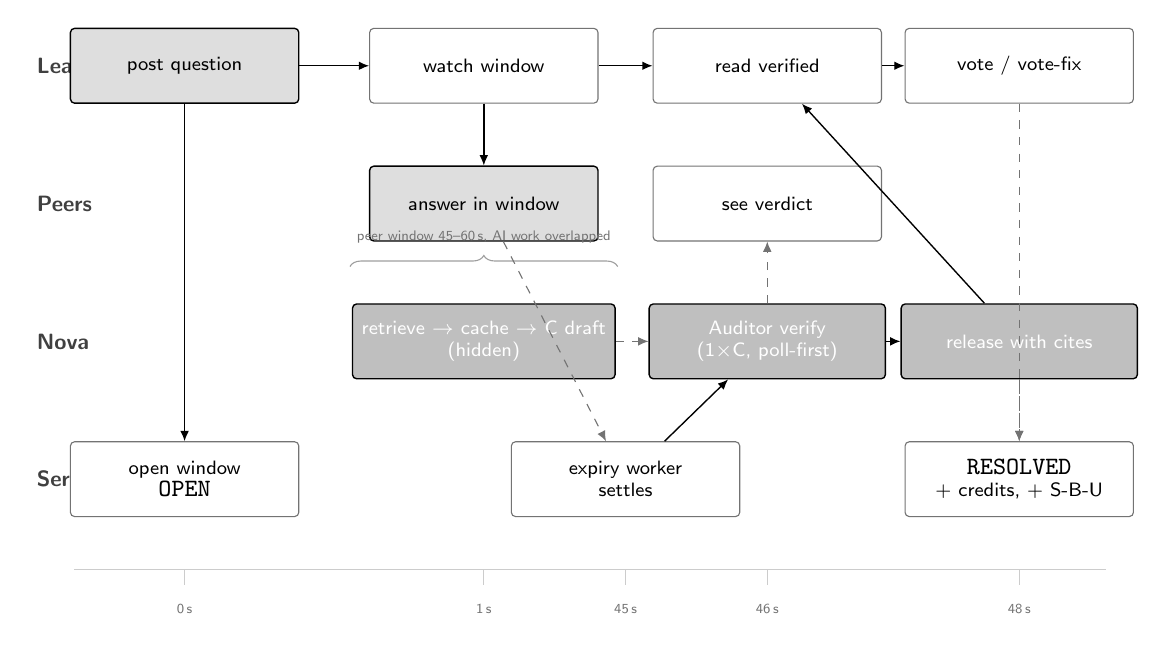
\begin{tikzpicture}[
  font=\sffamily\scriptsize,
  act/.style={draw=ink2,fill=white,rounded corners=1.5pt,minimum height=9.5mm,
              minimum width=29mm,align=center,line width=0.4pt},
  wact/.style={draw=ink0,fill=fillB,rounded corners=1.5pt,minimum height=9.5mm,
              minimum width=29mm,align=center,line width=0.5pt},
  ai/.style={draw=ink0,fill=fillC,text=white,rounded corners=1.5pt,minimum height=9.5mm,
             minimum width=30mm,align=center,line width=0.5pt},
  ar/.style={-{Latex[length=1.3mm,width=1.1mm]},draw=ink0,line width=0.5pt},
  dr/.style={-{Latex[length=1.3mm,width=1.1mm]},draw=ink2,line width=0.4pt,dashed},
  lane/.style={font=\sffamily\footnotesize\bfseries,color=ink1},
  tm/.style={font=\sffamily\tiny,color=ink2},
]
% lanes
\node[lane,anchor=west] at (-0.4,0) {Learner};
\node[lane,anchor=west] at (-0.4,-1.75) {Peers};
\node[lane,anchor=west] at (-0.4,-3.5) {Nova};
\node[lane,anchor=west] at (-0.4,-5.25) {Server};

% learner
\node[wact] (l1) at (1.6,0) {post question};
\node[act]  (l2) at (5.4,0) {watch window};
\node[act]  (l3) at (9.0,0) {read verified};
\node[act]  (l4) at (12.2,0) {vote / vote-fix};

% peers
\node[wact] (p1) at (5.4,-1.75) {answer in window};
\node[act]  (p2) at (9.0,-1.75) {see verdict};

% nova
\node[ai] (n1) at (5.4,-3.5) {retrieve $\to$ cache $\to$ C draft\\(hidden)};
\node[ai] (n2) at (9.0,-3.5) {Auditor verify\\(1$\times$C, poll-first)};
\node[ai] (n3) at (12.2,-3.5) {release with cites};

% server
\node[act] (s1) at (1.6,-5.25) {open window\\ \code{OPEN}};
\node[act] (s2) at (7.2,-5.25) {expiry worker\\ settles};
\node[act] (s3) at (12.2,-5.25) {\code{RESOLVED}\\ + credits, + S-B-U};

% timeline
\draw[ink4,line width=0.4pt] (0.2,-6.4) -- (13.3,-6.4);
\foreach \x/\t in {1.6/0\,s, 5.4/1\,s, 7.2/45\,s, 9.0/46\,s, 12.2/48\,s}{
  \draw[ink4] (\x,-6.4) -- (\x,-6.6);
  \node[tm] at (\x,-6.9) {\t};
}
\draw[decorate,decoration={brace,amplitude=4pt,mirror},ink3]
  (7.1,-2.55) -- (3.7,-2.55) node[midway,above=5pt,font=\sffamily\tiny,color=ink2]
  {peer window 45--60\,s, AI work overlapped};

\draw[ar] (l1) -- (l2);
\draw[ar] (l2) -- (l3);
\draw[ar] (l3) -- (l4);
\draw[ar] (l1) -- (s1);
\draw[ar] (l2) -- (p1);
\draw[dr] (p1) -- (s2);
\draw[ar] (s2) -- (n2);
\draw[dr] (n1) -- (n2);
\draw[ar] (n2) -- (n3);
\draw[ar] (n3) -- (l3);
\draw[dr] (n2) -- (p2);
\draw[dr] (n3) -- (s3);
\draw[dr] (l4) -- (s3);
\end{tikzpicture}
\caption{Circle-First Ask. The peer window is the only interval in which humans speak; the
model work is overlapped with it, so the AI answer is ready at the moment the window
closes. The withholding rule is enforced by question state, not by prompt instruction.}
\label{fig:cfas}
\end{figure}

\paragraph{Question state machine.} The withholding rule is a property of persisted state,
which is what makes it trustworthy. A question is \code{OPEN} while peers may answer;
\code{NOVA\_THINKING} after settlement begins, when the Quick Take is already written but
not yet exposed; and \code{RESOLVED} when the verified answer, its citations and any poll
are readable. The private and public views are separate routes, so a client cannot obtain
the hidden answer by reading a field it was not given: the public state route strips it,
and the private route is asker-only.

\paragraph{Pipeline stages.} Progress is reported as an ordered list of stages
(\code{retrieving}, \code{checking\_similar}, \code{writing}, \code{verifying}), each with
a start and completion timestamp. Responses arrive whole rather than streamed, so the
interface communicates staged progress instead of a partially-rendered answer
(\S\ref{sec:latency-ux}).

\section{Why the window is server-authoritative}

A tempting shortcut is to run the countdown in the browser. We rejected it for two
reasons visible in production. First, a client clock is untrusted and a backgrounded tab
throttles timers, so a window could outlive its deadline and peers would keep voting on
a settled question. Second, a single process restart in the middle of a window would
leave the question open forever, which is a visible product defect: the learner sees a
window that never closes.

The implementation therefore keeps the deadline on the server (\code{windowEndsAt} as an
indexed field), settles from a timer, and \emph{also} sweeps periodically so that a window
that expired while the process was down is settled on the next tick rather than never.
Clients derive their countdown from \code{windowEndsAt}, not from a server-provided
``now'', which also keeps conditional-GET validators stable:

\begin{lstlisting}[language=Java,caption={Dual settlement path: timer for the normal case, periodic sweep for the crash case.}]
/** Periodic sweep, so a window that expired while this process was down --
 *  or between a timer being set and a deploy -- is still settled. */
const overdue = await this.questions.find({ state: 'OPEN', windowEndsAt: { $lte: new Date() } });
const upcoming = await this.questions.find({ state: 'OPEN', windowEndsAt: { $gt: new Date() } });
for (const q of upcoming) this.schedule(q._id, +q.windowEndsAt - Date.now());
\end{lstlisting}

The same reasoning applies at deploy time: shutdown hooks drain in-flight requests and
clear the timers, so a deploy does not settle windows from a process that is already
dead. Settlement is idempotent, so a double settle cannot double-credit.

\section{Cross-cutting concerns}

\begin{table}[htbp]
\centering
\caption{Where each cross-cutting concern is implemented, and how it is enforced.}
\label{tab:crosscut}
\footnotesize
\begin{tabularx}{\textwidth}{@{}p{2.7cm}X p{4.3cm}@{}}
\toprule
\textbf{Concern} & \textbf{Implementation} & \textbf{Enforcement} \\
\midrule
Authentication & HMAC bearer token with learner ID, role and a token epoch
  & Default-deny guard; epoch bump invalidates all devices on passphrase change \\
Authorization & Role decorator plus circle-membership check
  & \code{authz-matrix} integration test: learner $\times$ mentor $\times$ admin
    $\times$ anonymous $\times$ cross-circle \\
Rate limiting & Named budgets (AI 10/min, writes 30/min, join-code 60/min per IP)
  & In-memory guard, with the edge limiter documented as the production layer \\
Validation & Zod-validated config at boot; \code{ValidationPipe} with
  \code{whitelist} and \code{forbidNonWhitelisted} on every route
  & Rejects unknown fields rather than ignoring them \\
Error contract & Uniform \code{\{error, code, retryable, user\_msg[4]\}}
  & Localized message asserted for all four languages in unit tests \\
Observability & Request-ID middleware, JSON logger, prom-client registry, event bus
  & \code{/metrics} key set asserted by the live smoke \\
Persistence & Mongoose schemas, 22 indexes, a two-migration registry, unit-of-work
  for transactions
  & Migrations are idempotent and indexed \\
Shutdown & \code{enableShutdownHooks}, timers drained, Mongo closed
  & Deploy smoke check \\
\bottomrule
\end{tabularx}
\end{table}

\section{Technology choices}

Each choice below was made against a constraint rather than by preference, and each is
justified by what it enabled.

\paragraph{NestJS 11 with TypeScript in strict mode.} The feature set is large enough that
module boundaries matter: 25 modules that can depend on \code{domain/} but not on the
adapter is a rule a framework can express and a flat Express app cannot. Strict mode with
no implicit \code{any} was decisive for a codebase that passes \code{unknown} model output
around: every parse of a model response is forced through a narrowing function, which is
where several real bugs were found.

\paragraph{MongoDB 8 with Mongoose.} Session state is document-shaped --- a question
carries its stages, its citations and its Quick Take together --- and a session reads as
one document rather than a join of six tables. Mongo also provides the two operational
properties this project depends on: TTL indexes for telemetry retention and atomic
\code{findOneAndUpdate} for quota reservation, which is what makes the governor correct
across concurrent requests.

\paragraph{React 19 with Vite and a PWA plugin.} A shared-device, campus-network context
wants an installable shell and a precached offline pack. Vite's build plus
\code{vite-plugin-pwa} produced both without a bespoke service worker.

\paragraph{TF-IDF retrieval instead of an embedding index.} This is the most debatable
choice, and it was made deliberately. A 39-chunk knowledge base over two topics does not
need embeddings to be retrieved well, and a local index has three properties a remote
embedding service does not: it builds in under a second at boot, it costs nothing per
query, and it keeps the grounded path alive in the \code{RED} and \code{BLACK} degradation
states. The trade-off is recall on paraphrases, which the three-variant query rewrite
partly compensates (\S\ref{sec:rag}).

\paragraph{A single provider adapter.} All model access goes through one file exposing
\code{compact}, \code{larger} and \code{available(tier)}. Two benefits follow: the product
can survive a provider change or a move to self-hosted open-weight models without touching
feature code, and the isolation is testable rather than aspirational.

\chapter{The Generative AI Layer}
\label{ch:ai}

This chapter documents the part of the system that is genuinely about generative AI:
how a turn is classified, how knowledge is retrieved and cited, how the hint ladder and
the Auditor are built to bound model usage, and how the whole layer degrades when the
model is not there. The organising principle throughout is that \emph{the model is the
most expensive and least reliable component}, so every use of it is a deliberate budgeted
decision with a template-based fallback.

\section{Group Pulse: one call, many decisions}

Per learner turn, the system needs four pieces of information: the intent of the message,
the language and register it was written in, whether it contains unsafe content or PII,
and how difficult the underlying question is. The naive implementation makes four calls.
HALQA makes one schema-constrained compact call and shares its result across four
consumers.

\begin{table}[htbp]
\centering
\caption{The Group Pulse schema and its consumers. One compact call per turn window serves
credits, confusion tracking, register detection and the difficulty gate.}
\label{tab:pulse}
\footnotesize
\begin{tabularx}{\textwidth}{@{}p{3.1cm}p{3.0cm}X@{}}
\toprule
\textbf{Field} & \textbf{Domain} & \textbf{Consumed by} \\
\midrule
\code{intent} & \code{ask}, \code{explain}, \code{help\_offer}, \code{dispute},
  \code{chitchat}, \code{meta} & Router (task selection) and credit weights
  (\S\ref{sec:credits}) \\
\code{helpful\_0\_2} & $0..2$ & Credit award for explanations; S-B-U \emph{Build} ring \\
\code{bridging\_bool} & boolean & Connects two learners' ideas; \emph{Bridge Builder} badge \\
\code{skeptic\_bool} & boolean & Kind-skeptic credit; disagreement is data, not shame \\
\code{confusion\_0\_1} & $0..1$ & Confusion signal; drives hint eagerness and
  \code{needs\_human} \\
\code{lang} & \code{ar}, \code{darija}, \code{fr}, \code{en} & Response register and
  retrieval language filter \\
\bottomrule
\end{tabularx}
\end{table}

Two implementation details matter for correctness under latency. First, the response is
parsed through a narrowing function that validates every field and substitutes a safe
default (\code{chitchat}, neutral helpfulness) rather than throwing: a malformed model
reply must degrade one turn, not fail the request. Second, the call is guarded so that
\emph{at most one} Group Pulse runs per turn window; a burst of messages collapses into a
single classification. Both are unit-tested in \code{router-pure.spec.ts}.

\section{Retrieval-augmented generation}
\label{sec:rag}

\subsection{The knowledge base}

Knowledge lives in versioned JSON seed files rather than in a vector store, because the
corpus is small, curated and needs to be auditable. This submission ships two packs ---
\emph{binary search} and \emph{fractions} --- totalling 39 chunks, each with a stable
identifier, a language, a kind, and an explicit list of \emph{claims} it supports.

\begin{table}[htbp]
\centering
\caption{Knowledge base composition. Every chunk carries claim checklists, which is what
lets the Auditor verify a peer answer without a second retrieval pass.}
\label{tab:kb}
\footnotesize
\begin{tabular}{@{}lrrrr@{}}
\toprule
\textbf{Pack} & \textbf{Chunks} & \textbf{ar} & \textbf{darija} & \textbf{fr / en} \\
\midrule
\code{binary\_search.json} & 27 & 6 & 6 & 15 \\
\code{fractions.json}      & 12 & 1 & 1 & 10 \\
\midrule
\textbf{Total}             & \textbf{39} & 7 & 7 & 25 \\
\bottomrule
\end{tabular}
\end{table}

The manifest \code{kb/SOURCES.md} lists every chunk identifier with its provenance and
licence, and a test asserts that the seed files and the manifest agree in both
directions --- a chunk listed but not shipped, or shipped but not listed, fails the build.
All content is team-written and synthetic, which also means the data sent to the provider
contains no third-party material and no learner data.

\subsection{Index and query}

Chunks are indexed at boot with TF-IDF over a normalised token field. The index builds in
under a second, which is what allows it to be rebuilt on every process start with no
persistence layer and no warm-up window.

Each grounded query is rewritten into three template variants (base, base with the level
appended, base with an example cue appended), every variant is scored, results are
deduplicated by chunk identifier keeping the best score, ties are broken deterministically
by identifier, and the top five are attached to the prompt together with their claim
checklists.

\begin{lstlisting}[language=Java,caption={Query across the three rewrite variants, with deterministic dedupe.}]
search(intent, level, sessionLang, topK = 5) {
  const norm = normaliseArabizi(intent);
  const best = new Map();
  for (const variant of rewriteQuery(norm, level)) {
    for (const hit of this.index.search(variant, sessionLang, topK)) {
      // keep the best score per chunk, so expansion can only help recall
      const prev = best.get(hit.chunkId);
      if (!prev || hit.score > prev.score) best.set(hit.chunkId, hit);
    }
  }
  return [...best.values()]
    .sort((a, b) => b.score - a.score || (a.chunkId < b.chunkId ? -1 : 1))
    .slice(0, topK);
}
\end{lstlisting}

Determinism here is not aesthetic. The demo, the evals and the smoke test all compare
outputs across runs, so retrieval that varied between runs would make every downstream
assertion flaky. Sorting ties by identifier also means the escalation gate --- which counts
\emph{conflicting} chunks --- sees a stable set.

\subsection{Mandatory citations}

Every grounded answer must cite chunk identifiers, and the interface renders them as
citation chips beneath the answer. This is a stronger requirement than it looks: a
citation is only useful if the claim it supports is checkable, so the same claim
checklists that are attached to the prompt are stored with the answer and later used by
the Auditor to verify peer claims. One artefact, three consumers --- grounding,
verification and the offline pack.

\begin{note}[Why citations reduce load rather than increase it]
An answer with five citations is longer, but it is also more likely to be accepted without
a follow-up question, which is the expensive path. In practice the citation obligation is a
token cost paid once to avoid a second turn, and it makes the Auditor's job a set
comparison rather than a fresh generation.
\end{note}

\subsection{Arabizi normalisation}
\label{sec:arabizi}

Tunisian learners routinely write Darija in Latin script with digits standing in for
letters: \code{3} for \emph{ain}, \code{7} for \emph{ha}, \code{9} for \emph{qaf}, and
\code{5} or \code{kh} for \emph{kha}. Two learners can ask the same question in Arabic
script and in Arabizi, and a tokenizer that treats them as unrelated strings will fail to
retrieve the same chunk for both.

The domain layer therefore ships a pure normaliser and a register detector. Detection runs
before retrieval so that a chunk in the wrong register is never attached to a prompt: a
Darija question receives Darija chunks. Because the functions are pure and
dependency-free, they are tested on a fixed corpus of real orthographic variants, and the
same code path is reused by the cache key builder so that an equivalent re-ask in a
different encoding can still hit the cache.

\section{The hint ladder}
\label{sec:hints}

The ladder is the mechanism by which the system \emph{scaffolds rather than solves}. Four
levels escalate from a nudge to a full worked solution, and the passport decides how early
the ladder may begin for a given learner.

\begin{table}[htbp]
\centering
\caption{The four hint levels, all served at zero model cost except the last.}
\label{tab:ladder}
\footnotesize
\begin{tabularx}{\textwidth}{@{}p{1.0cm}p{2.5cm}X p{3.3cm}@{}}
\toprule
\textbf{Level} & \textbf{Kind} & \textbf{Content} & \textbf{Source} \\
\midrule
L1 & Nudge & A question that names the missing precondition without stating it:
   \emph{``What must be true about the array before you start halving?''} & T0 template \\
L2 & Analogy & A concrete counter-example that breaks the learner's current mental model:
   \emph{``Is the list [5,1,4] sorted? Try one halving step and see what breaks.''}
   & T0 template \\
L3 & Worked start & The first step of a \emph{different} instance, so the learner
   transfers the move rather than copying the answer & T0 template \\
L4 & Full solution & The hidden Quick Take, with citations & Prepared during the peer
   window \\
\bottomrule
\end{tabularx}
\end{table}

L1--L3 are templates keyed by topic and language. They cost nothing, they cannot fail, and
they are available in every degradation state including \code{BLACK}. L4 is the prepared
answer, and it is \emph{leak-gated in code}: the service refuses L4 unless the learner has
already advanced the hint state to at least level three or pressed skip. The guard is a
condition on persisted state, not an instruction in a prompt, and a unit test asserts the
refusal:

\begin{lstlisting}[language=Java,caption={The L4 leak gate. A prompt-only instruction would be advisory; this is not.}]
// T0 leak gate (enforced in code, not prompt): L4 requires hintState >= 3
if (level === 4 && !(q.hintState >= 3 || q.skipPressed)) throw Err.denied('HINT_L4_LOCKED');
\end{lstlisting}

The gate exists because a ladder that can be short-circuited is not a ladder. If a learner
could request L4 immediately, the scaffolding would be decorative and the system would
revert to an answer machine.

\section{The Auditor}
\label{sec:auditor}

Peers first creates a new failure mode: the group can now converge confidently on a wrong
answer. The Auditor exists to prevent that, and its design is shaped by the quota
constraint --- verification must be cheap enough to run on every settled question.

\begin{figure}[htbp]
\centering
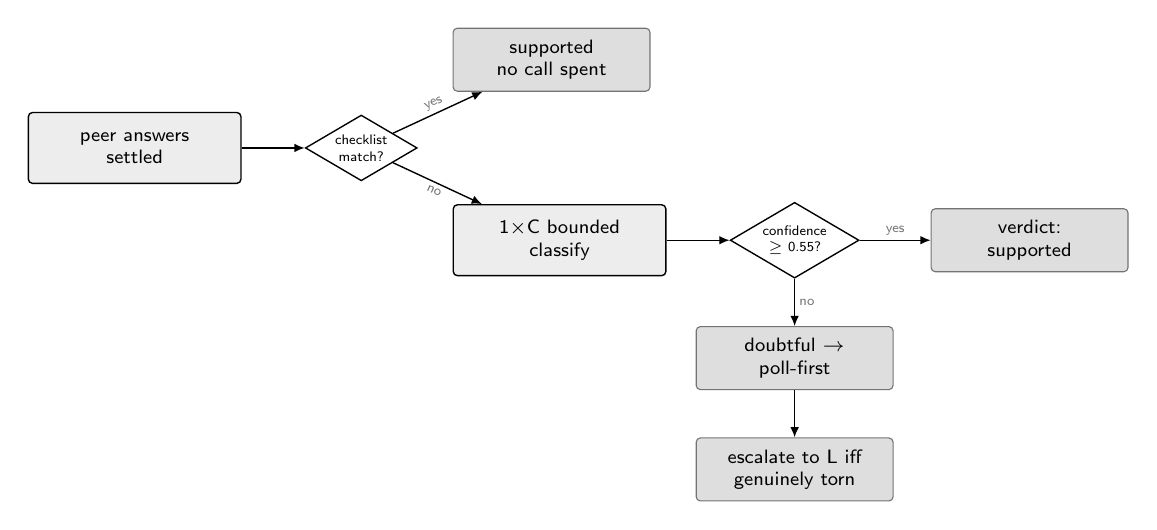
\begin{tikzpicture}[
  font=\sffamily\scriptsize,
  st/.style={draw=ink0,fill=fillA,rounded corners=1.5pt,minimum height=9mm,
             minimum width=27mm,align=center,line width=0.5pt},
  dec/.style={draw=ink0,fill=white,shape=diamond,aspect=1.7,inner sep=1pt,
              align=center,line width=0.5pt,font=\sffamily\tiny},
  resx/.style={draw=ink2,fill=fillB,rounded corners=1.5pt,minimum height=8mm,
              minimum width=25mm,align=center,line width=0.4pt},
  ar/.style={-{Latex[length=1.3mm,width=1.1mm]},draw=ink0,line width=0.5pt},
  lbl/.style={font=\sffamily\tiny,color=ink2,inner sep=1.5pt},
]
\node[st] (in) {peer answers\\settled};
\node[dec,right=8mm of in] (cheap) {checklist\\match?};
\node[resx,above right=5mm and 8mm of cheap] (verdict) {supported\\no call spent};
\node[st,below right=5mm and 8mm of cheap] (clf) {1$\times$C bounded\\classify};
\node[dec,right=8mm of clf] (conf) {confidence\\$\ge$ 0.55?};
\node[resx,right=9mm of conf] (ok) {verdict:\\supported};
\node[resx,below=6mm of conf] (poll) {doubtful $\to$\\poll-first};
\node[resx,below=6mm of poll] (esc) {escalate to L iff\\genuinely torn};

\draw[ar] (in) -- (cheap);
\draw[ar] (cheap) -- node[lbl,above,sloped] {yes} (verdict);
\draw[ar] (cheap) -- node[lbl,below,sloped] {no} (clf);
\draw[ar] (clf) -- (conf);
\draw[ar] (conf) -- node[lbl,above,sloped] {yes} (ok);
\draw[ar] (conf) -- node[lbl,right] {no} (poll);
\draw[ar] (poll) -- (esc);
\end{tikzpicture}
\caption{Auditor verification order. The cheap path is attempted first: a checklist match
settles the question with no model call at all. Confidence below the configured threshold
yields a poll rather than a counter-assertion.}
\label{fig:auditor}
\end{figure}

Three properties of this design are worth stating explicitly.

\paragraph{Cheap path first.} Peer answers are compared against the claim checklist of the
retrieved chunks. Where a claim is directly supported or directly contradicted, the verdict
costs nothing. Only disagreement that the checklist cannot settle reaches the model.

\paragraph{Poll before assertion.} When the Auditor is doubtful, it does not override the
peer. It opens a consensus poll on the contested claim, and the group votes. This
preserves the design position --- the circle decides, the AI structures the decision ---
and it converts an AI judgement into a collective one, which is also the pedagogically
better outcome.

\paragraph{Escalation is explicit.} A low compact-tier confidence sets an escalation flag
rather than silently invoking the larger model. The flag is what the router reads, so the
larger-tier budget is spent by a recorded decision with a recorded reason.

\section{The learning-DNA passport}
\label{sec:dna}

Personalization in this system is a small number of well-chosen questions and a long
half-life for their answers. The diagnostic is four items, designed to complete in under
three minutes on a phone, and each item changes a specific downstream behaviour.

\begin{table}[htbp]
\centering
\caption{The four diagnostic items and the state each one writes.}
\label{tab:dna}
\footnotesize
\begin{tabularx}{\textwidth}{@{}p{0.9cm}p{3.6cm}p{2.5cm}X@{}}
\toprule
\textbf{Item} & \textbf{Prompt (trilingual)} & \textbf{Writes} & \textbf{Effect} \\
\midrule
L1 & Level in the current topic: novice / beginner / intermediate
   & \code{level}, \code{levelByTopic} & Chunk level filter; ladder starting point;
     difficulty gate \\
S1 & What helps most: a picture, a daily-life analogy, or numbered steps
   & \code{styleWeights} & Initial weights over six styles; retrieval variant selection \\
G1 & Preferred register: Arabic, Darija, French, English
   & \code{lang} & Response register, chunk language filter, UI locale \\
C1 & Confidence: sure / unsure / lost
   & \code{hintEagerness} & Ladder eagerness ($0.3 / 0.6 / 0.9$); invite flag \\
\bottomrule
\end{tabularx}
\end{table}

The style dimensions are six rather than three (\code{visual}, \code{analogy},
\code{steps}, \code{example}, \code{repetition}, \code{practice}) because the diagnostic
can only \emph{anchor} a prior, not determine a learner. After each check-question the
bandit performs one documented update.

\begin{figure}[htbp]
\centering
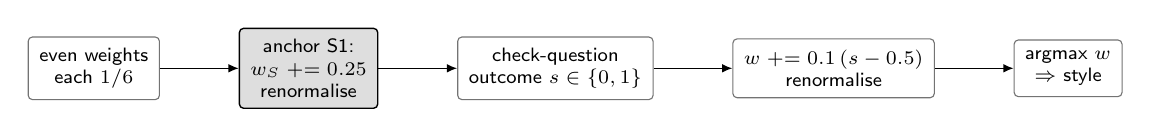
\begin{tikzpicture}[
  font=\sffamily\scriptsize,
  ar/.style={-{Latex[length=1.3mm,width=1.1mm]},draw=ink0,line width=0.5pt},
  bx/.style={draw=ink2,fill=white,rounded corners=1.5pt,inner sep=4pt,align=center,
             line width=0.4pt},
  hl/.style={draw=ink0,fill=fillB,rounded corners=1.5pt,inner sep=4pt,align=center,
             line width=0.5pt},
]
\node[bx] (start) {even weights\\each $1/6$};
\node[hl,right=10mm of start] (anchor) {anchor S1:\\$w_S \mathrel{+}= 0.25$\\renormalise};
\node[bx,right=10mm of anchor] (check) {check-question\\outcome $s\in\{0,1\}$};
\node[bx,right=10mm of check] (upd) {$w \mathrel{+}= 0.1\,(s-0.5)$\\renormalise};
\node[bx,right=10mm of upd] (pick) {argmax $w$\\$\Rightarrow$ style};
\draw[ar] (start) -- (anchor);
\draw[ar] (anchor) -- (check);
\draw[ar] (check) -- (upd);
\draw[ar] (upd) -- (pick);
\end{tikzpicture}
\caption{Style adaptation. The passport supplies a prior; a single documented bandit step
per check-question moves it. Weights always sum to one and never fall below a floor, so a
style cannot be permanently extinguished by early bad luck.}
\label{fig:bandit}
\end{figure}

The update is $\alpha = 0.1$ against a baseline of $0.5$, with a floor of $0.01$ per style
followed by renormalisation. The floor matters: without it, a learner who has two unlucky
visual explanations in a row could drive \code{visual} near zero and never see a diagram
again, which is a worse error than the one the bandit was correcting.

\section{The Whisper relay (teach to learn)}
\label{sec:whisper}

Explaining is the highest-value learner activity in the system, and it is also where
misconceptions become visible. The Whisper relay asks a learner to paraphrase a chain of at
least two links, then compares the paraphrase against the claim checklist of the source
chunks and reports a \emph{drift map} with four categories:

\begin{itemize}[leftmargin=1.4em,itemsep=1pt]
  \item \textbf{kept} --- claims reproduced correctly;
  \item \textbf{lost} --- claims present in the source and absent from the paraphrase;
  \item \textbf{distorted} --- claims reproduced with a changed meaning;
  \item \textbf{added} --- claims asserted that the sources do not support.
\end{itemize}

A T0 comparison runs first and settles obvious cases; only a genuinely ambiguous chain
reaches a compact call. The chain must have at least two links, which is validated
server-side rather than trusted from the client --- a one-link ``chain'' is a learner
copying a sentence, not explaining it. After the drift map, the learner gets exactly one
repair round: the pedagogic value is in repairing the distortion, not in being graded on it.

\section{Engineered behaviour under limited capacity}
\label{sec:degradation}

This is the section the design position most directly determines. If the AI must not
replace the circle, then losing the AI must not end the session. The system therefore
models availability as four states, and each state changes what the interface
\emph{promises}.

\begin{figure}[htbp]
\centering
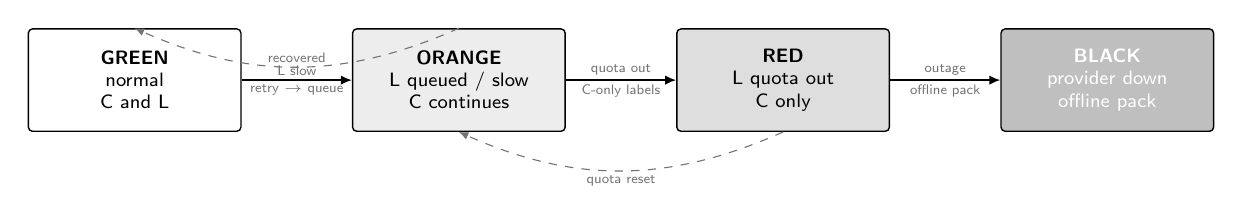
\begin{tikzpicture}[
  font=\sffamily\scriptsize,
  st/.style={draw=ink0,minimum height=13mm,minimum width=27mm,align=center,
             line width=0.5pt,rounded corners=1.5pt},
  g/.style={st,fill=white},
  o/.style={st,fill=fillA},
  r/.style={st,fill=fillB},
  b/.style={st,fill=fillC,text=white},
  ar/.style={-{Latex[length=1.4mm,width=1.2mm]},draw=ink0,line width=0.6pt},
  back/.style={-{Latex[length=1.2mm,width=1.0mm]},draw=ink2,line width=0.4pt,dashed,bend left=24},
  lbl/.style={font=\sffamily\tiny,color=ink2,align=center,inner sep=1.5pt},
]
\node[g] (green) {\textbf{GREEN}\\ normal\\ C and L};
\node[o,right=14mm of green] (orange) {\textbf{ORANGE}\\ L queued / slow\\ C continues};
\node[r,right=14mm of orange] (red) {\textbf{RED}\\ L quota out\\ C only};
\node[b,right=14mm of red] (black) {\textbf{BLACK}\\ provider down\\ offline pack};

\draw[ar] (green) -- node[lbl,above] {L slow} node[lbl,below] {retry $\to$ queue} (orange);
\draw[ar] (orange) -- node[lbl,above] {quota out} node[lbl,below] {C-only labels} (red);
\draw[ar] (red) -- node[lbl,above] {outage} node[lbl,below] {offline pack} (black);
\draw[back] (orange.north) to node[lbl,above] {recovered} (green.north);
\draw[back] (red.south) to node[lbl,below] {quota reset} (orange.south);
\end{tikzpicture}
\caption{The degradation machine. Every transition emits a UI banner, a telemetry event and
a metric gauge, and every state is rehearsable through a development-only chaos toggle.}
\label{fig:degradation}
\end{figure}

\begin{table}[htbp]
\centering
\caption{What each degradation state changes, stated as a product promise.}
\label{tab:degstates}
\footnotesize
\begin{tabularx}{\textwidth}{@{}p{1.55cm}X p{4.2cm}@{}}
\toprule
\textbf{State} & \textbf{Promise kept} & \textbf{Mechanism} \\
\midrule
GREEN  & Full quality, both tiers, citations, capsule polishing
       & Normal routing \\
ORANGE & Peers still first and the session still works; the deeper answer arrives with a
         position and an ETA & L requests enter the FIFO queue with position and ETA
         surfaced; one guided retry, then C fallback \\
RED    & Every question still gets a grounded compact-tier answer with simplified labels;
         no feature disappears silently & L reservations refused atomically; the router
         downgrades; labels and prose are simplified \\
BLACK  & The circle continues with peer work, polls, role-play and flashcards from a
         30-snippet offline pack; nothing is lost & Offline pack served with an
         \code{offline:true} label; writes queued for later sync \\
\bottomrule
\end{tabularx}
\end{table}

\subsection{The quota governor}

The governor is the component that makes the state machine real rather than advisory. It
maintains two ledgers --- per session and per circle per day --- and reserves atomically,
because the obvious implementation is wrong in a way that only appears under load.

\begin{lstlisting}[language=Java,caption={Reserve then compare. Checking before incrementing lets N replicas each read ``under cap'' and all spend.}]
// Increment first, then compare: check-then-increment lets N replicas each read
// "under the cap" and all spend, which is exactly the failure this exists to prevent.
const reservedField = tier === 'C' ? '$reservedC' : '$reservedL';
const capField     = tier === 'C' ? '$cCap'      : '$lCap';
\end{lstlisting}

A single circle can open many sessions in a day, so a per-session cap alone does not bound
a class: ten squads of four against a 20-call session cap is already 200 calls. The
per-circle daily ceiling (\code{CIRCLE\_DAILY\_CALLS}, default 400) is the binding limit,
and it sits above normal classroom use and below a runaway loop.

\subsection{Semantic cache}

Cache keys are a SHA-1 digest over the normalised intent, the level, the language, the
sorted chunk identifiers and the ladder state. The normaliser strips case, diacritics and a
multilingual stop-word list,
so equivalent re-asks collapse to one key and are served without a model call. This is the
cheapest possible win on the ``fewer, well-built requests'' objective, and it is metered:
\code{cacheHitRate} is a first-class metric, not an internal counter.

\subsection{Latency UX}
\label{sec:latency-ux}

Because responses arrive whole rather than streamed, the interface cannot show a partial
answer, and faking a token stream would misrepresent what the system knows. Instead:

\begin{enumerate}[leftmargin=1.6em,itemsep=2pt]
  \item a zero-model-call skeleton renders in under 200\,ms, so the section is never empty;
  \item the compact tier fills the sections it owns;
  \item the larger tier, when it was escalated, slides in afterwards and is labelled
        \emph{deeper answer ready}.
\end{enumerate}

Progress inside a single turn is communicated as the ordered pipeline stages
(\S\ref{sec:cfas}), so the learner sees \emph{retrieving} then \emph{verifying} rather than
a spinner with no semantics.

\chapter{Backend Design}
\label{ch:backend}

\section{Module map}

The API is organised into 25 feature modules. The grouping below is the one used in
code review, because it separates the modules that decide \emph{what the AI may do} from
the ones that decide \emph{what the learner sees}.

\begin{table}[htbp]
\centering
\caption{The 25 backend modules grouped by responsibility.}
\label{tab:modules}
\footnotesize
\begin{tabularx}{\textwidth}{@{}p{3.0cm}X@{}}
\toprule
\textbf{Group} & \textbf{Modules} \\
\midrule
Session core & \code{session}, \code{circle}, \code{question}, \code{peer-window},
  \code{workshop} --- circles, membership, the question state machine and the
  server-authoritative window \\
AI platform & \code{learning} (DNA and bandit), \code{hints}, \code{auditor},
  \code{consensus}, \code{whisper}, \code{capsule}, \code{quiz}, \code{coach} --- the
  generative surface \\
Learner surfaces & \code{solo}, \code{gamification}, \code{equity}, \code{matcher} ---
  individual practice, credits, fairness and circle composition \\
Facilitation & \code{mentor}, \code{dashboard}, \code{sbu}, \code{projections},
  \code{analytics} --- the board, health rings and metrics \\
Platform & \code{auth}, \code{knowledge}, \code{offline}, \code{settings} --- identity,
  retrieval corpus, offline pack and configuration \\
\bottomrule
\end{tabularx}
\end{table}

Each module follows the same internal shape: a controller that validates and authorizes, a
service that owns the use case, and direct schema access through the model registry. There
is no repository layer, deliberately: with 18 collections and no cross-service query
composition beyond two joins that already live in a projection, a repository layer would
add indirection without adding a seam.

\section{Domain layer}

The \code{domain/} directory holds fifteen dependency-free modules. They are the parts of
the system that can be proven by example, and they carry most of the invariants the report
claims. Two of them deserve their formulas in full, because they encode product decisions.

\subsection{Credits with a logarithmic cap}
\label{sec:credits}

Participation credits reward quality, not volume, because a chatty learner must not
outrank a quiet one who asked the question that unlocked the group. Weights are
configured in \code{config/equity.yaml} and mirrored by a default table in code:

\begin{table}[htbp]
\centering
\caption{Credit weights and the volume cap.}
\label{tab:credits}
\footnotesize
\begin{tabular}{@{}lr@{\hspace{18pt}}lr@{}}
\toprule
\textbf{Action} & \textbf{Weight} & \textbf{Action} & \textbf{Weight} \\
\midrule
\code{sharp\_question}   & 3 & \code{poll\_vote}    & 1 \\
\code{good\_explanation} & 3 & \code{me\_too}       & 1 \\
\code{bridging}          & 3 & \code{scribe\_note}  & 1 \\
\code{kind\_skeptic}     & 3 & \code{plain\_message} & 0.5, log-capped \\
\bottomrule
\end{tabular}
\end{table}

Plain messages are capped logarithmically with $k=2$:
\begin{equation}
\mathrm{effective}_{\mathrm{plain}}(n) \;=\; 2\,\ln(1+n).
\label{eq:logcap}
\end{equation}

The worked example from the blueprint is the one the test asserts. Learner A posts twelve
plain messages: $2\ln 13 \approx 5.1$. Learner B asks one sharp question, makes one
bridging connection and casts one vote: $3+3+1 = 7$. B outranks A despite twelve times
fewer messages. Without the cap, A would score $6$ on weight alone and the reward would
train the wrong behaviour.

\subsection{S-B-U circle health}
\label{sec:sbu}

Each circle has three rings, computed from telemetry on every event. The names are
\emph{Structured}, \emph{Balanced} and \emph{Understood}; the formulas are fixed in
\code{config/sbu.yaml}:

\begin{align}
S &= 0.4\,a + 0.3\,t + 0.3\,r, \label{eq:s}\\
B &= 1 - \mathrm{dispersion}(\text{credits}), \label{eq:b}\\
U &= 0.5\,c + 0.3\,(1 - \bar{h}/3) + 0.2\,(1 - \kappa), \label{eq:u}
\end{align}

where $a$ is agenda completion, $t$ time discipline, $r$ recap completion, $c$ the
check-success rate, $\bar h$ the mean hint depth on a $0..4$ scale, and $\kappa$ the
corrections per answer, capped to $0..1$ upstream. Dispersion is the coefficient of
variation of credits across members, so a circle where one learner earns everything scores
$B \approx 0$ and a perfectly shared circle scores $B \approx 1$.

Ring display thresholds are $\ge 0.75$ \emph{bright}, $0.45$--$0.75$ \emph{steady}, below
$0.45$ \emph{pulse}. Neutral priors are used where a signal is not yet measurable
($t = 0.5$, $c = 0.5$), so a new circle is not punished for having no history. The
\code{needs\_human} flag fires when $B < 0.45$, $U < 0.45$, or a misconception has been
open for more than three minutes; it routes mentor attention rather than replacing it.

\subsection{Other domain modules}

\begin{table}[htbp]
\centering
\caption{Domain modules and the invariant each one owns.}
\label{tab:domain}
\footnotesize
\begin{tabularx}{\textwidth}{@{}p{3.2cm}X@{}}
\toprule
\textbf{Module} & \textbf{Invariant} \\
\midrule
\code{pii.ts} & Email, phone, address hints and long digit runs are redacted before any
  text leaves the process; the function returns findings, not a boolean, so a caller can
  tell the learner what was removed \\
\code{cache-key.ts} & Equivalent re-asks collapse to one key: normalise, sort chunk ids,
  include the ladder state \\
\code{arabizi.ts} & Register detection and Latin-digit transliteration normalisation,
  shared by retrieval and the cache \\
\code{bandit.ts} & Style weights sum to one, never fall below the floor, and update by
  one documented step \\
\code{credits.math.ts} & Credits are quality-weighted and log-capped; dispersion is a
  coefficient of variation \\
\code{sbu.math.ts} & The three rings, the display tiers and the \code{needs\_human}
  predicate \\
\code{confusion.ts} & Confusion signals, including the short-after-long pattern, with a
  documented primary signal \\
\code{ids.ts} & Learner identifiers match \code{L-\textbackslash d\{2,4\}}; no other
  format is accepted at any boundary \\
\code{hint-templates.ts} & L1--L3 exist for every supported topic and language, so the
  ladder can never be empty \\
\code{tokens.ts} & Token budgeting scales the caller's output request for reasoning
  models rather than assuming a fixed budget \\
\bottomrule
\end{tabularx}
\end{table}

\section{Data model}

Eighteen collections, seven schemas holding several definitions each, and 22 indexes
chosen for the three access patterns that matter: the state poller, the expiry worker and
the per-circle read.

\begin{figure}[htbp]
\centering
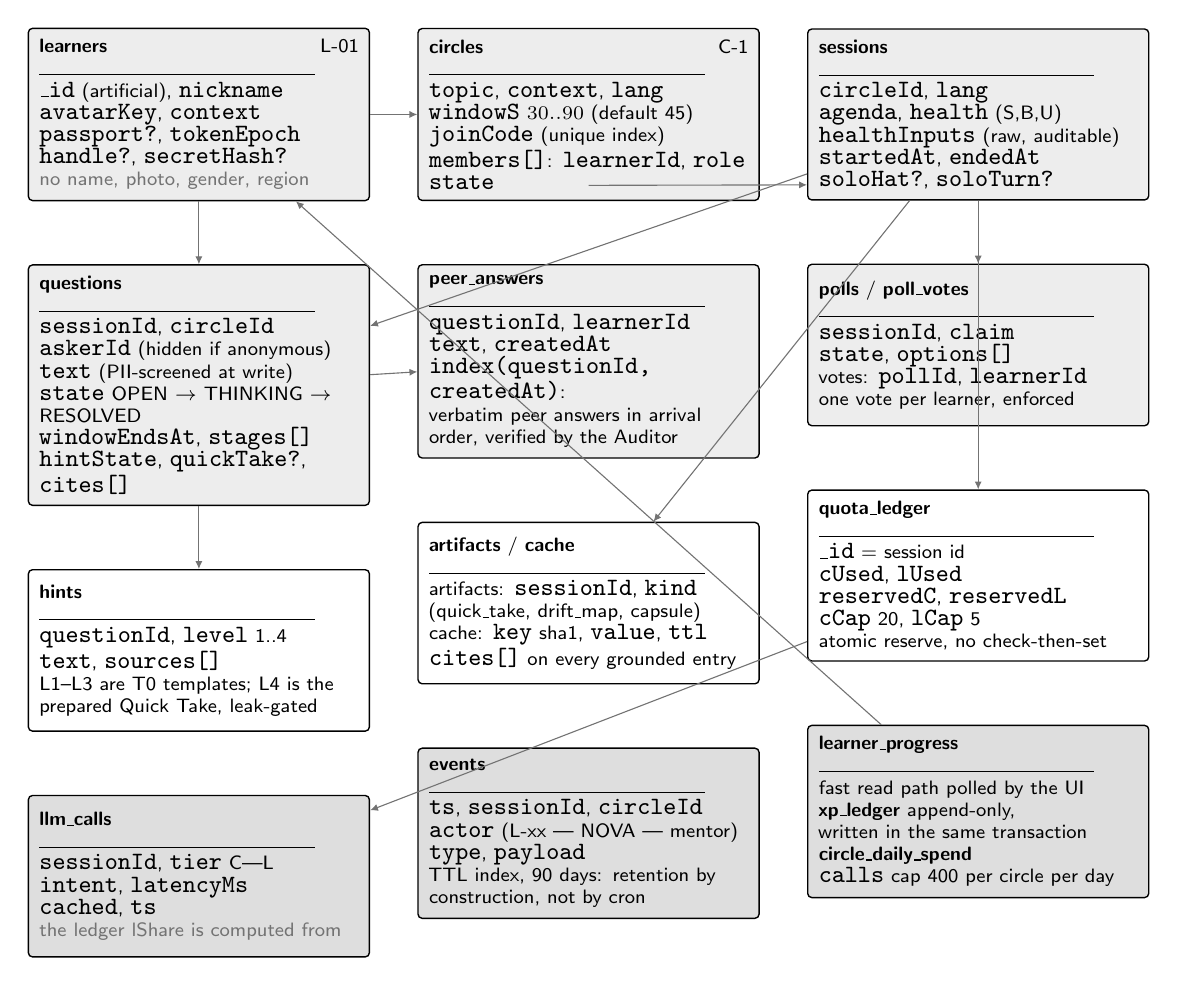
\begin{tikzpicture}[
  font=\sffamily\scriptsize,
  card/.style={draw=ink0,fill=fillA,rounded corners=1.5pt,align=left,inner sep=4pt,
               text width=4.05cm,line width=0.5pt,minimum height=2.05cm},
  cardw/.style={card,fill=white},
  cardd/.style={card,fill=fillB},
  rel/.style={draw=ink2,line width=0.4pt,-{Latex[length=1mm,width=0.9mm]}},
]
% row 1 -- identity and group
\node[card] (learner) {\textbf{learners} \hfill L-01\\
  \rule{3.5cm}{0.3pt}\\
  \code{\_id} (artificial), \code{nickname}\\
  \code{avatarKey}, \code{context}\\
  \code{passport?}, \code{tokenEpoch}\\
  \code{handle?}, \code{secretHash?}\\
  {\color{ink2}no name, photo, gender, region}};
\node[card,right=6mm of learner] (circle) {\textbf{circles} \hfill C-1\\
  \rule{3.5cm}{0.3pt}\\
  \code{topic}, \code{context}, \code{lang}\\
  \code{windowS} $30..90$ (default 45)\\
  \code{joinCode} (unique index)\\
  \code{members[]}: \code{learnerId}, \code{role}\\
  \code{state}};
\node[card,right=6mm of circle] (session) {\textbf{sessions}\\
  \rule{3.5cm}{0.3pt}\\
  \code{circleId}, \code{lang}\\
  \code{agenda}, \code{health} (S,B,U)\\
  \code{healthInputs} (raw, auditable)\\
  \code{startedAt}, \code{endedAt}\\
  \code{soloHat?}, \code{soloTurn?}};

% row 2 -- the interaction
\node[card,below=8mm of learner] (question) {\textbf{questions}\\
  \rule{3.5cm}{0.3pt}\\
  \code{sessionId}, \code{circleId}\\
  \code{askerId} (hidden if anonymous)\\
  \code{text} (PII-screened at write)\\
  \code{state} OPEN $\to$ THINKING $\to$ RESOLVED\\
  \code{windowEndsAt}, \code{stages[]}\\
  \code{hintState}, \code{quickTake?}, \code{cites[]}};
\node[card,below=8mm of circle] (peer) {\textbf{peer\_answers}\\
  \rule{3.5cm}{0.3pt}\\
  \code{questionId}, \code{learnerId}\\
  \code{text}, \code{createdAt}\\
  \code{index(questionId, createdAt)}:\\
  verbatim peer answers in arrival\\
  order, verified by the Auditor};
\node[card,below=8mm of session] (poll) {\textbf{polls} / \textbf{poll\_votes}\\
  \rule{3.5cm}{0.3pt}\\
  \code{sessionId}, \code{claim}\\
  \code{state}, \code{options[]}\\
  votes: \code{pollId}, \code{learnerId}\\
  one vote per learner, enforced};

% row 3 -- AI artefacts
\node[cardw,below=8mm of question] (hint) {\textbf{hints}\\
  \rule{3.5cm}{0.3pt}\\
  \code{questionId}, \code{level} 1..4\\
  \code{text}, \code{sources[]}\\
  L1--L3 are T0 templates; L4 is the\\
  prepared Quick Take, leak-gated};
\node[cardw,below=8mm of peer] (ai) {\textbf{artifacts} / \textbf{cache}\\
  \rule{3.5cm}{0.3pt}\\
  artifacts: \code{sessionId}, \code{kind}\\
  (quick\_take, drift\_map, capsule)\\
  cache: \code{key} sha1, \code{value}, \code{ttl}\\
  \code{cites[]} on every grounded entry};
\node[cardw,below=8mm of poll] (quota) {\textbf{quota\_ledger}\\
  \rule{3.5cm}{0.3pt}\\
  \code{\_id} = session id\\
  \code{cUsed}, \code{lUsed}\\
  \code{reservedC}, \code{reservedL}\\
  \code{cCap} 20, \code{lCap} 5\\
  atomic reserve, no check-then-set};

% row 4 -- operational
\node[cardd,below=8mm of hint] (llm) {\textbf{llm\_calls}\\
  \rule{3.5cm}{0.3pt}\\
  \code{sessionId}, \code{tier} C|L\\
  \code{intent}, \code{latencyMs}\\
  \code{cached}, \code{ts}\\
  {\color{ink2}the ledger lShare is computed from}};
\node[cardd,below=8mm of ai] (event) {\textbf{events}\\
  \rule{3.5cm}{0.3pt}\\
  \code{ts}, \code{sessionId}, \code{circleId}\\
  \code{actor} (L-xx | NOVA | mentor)\\
  \code{type}, \code{payload}\\
  TTL index, 90 days: retention by\\
  construction, not by cron};
\node[cardd,below=8mm of quota] (prog) {\textbf{learner\_progress}\\
  \rule{3.5cm}{0.3pt}\\
  fast read path polled by the UI\\
  \textbf{xp\_ledger} append-only,\\
  written in the same transaction\\
  \textbf{circle\_daily\_spend}\\
  \code{calls} cap 400 per circle per day};

% relations
\draw[rel] (learner) -- (circle);
\draw[rel] ([yshift=2mm]circle.south) -- ([yshift=2mm]session.south west);
\draw[rel] (learner) -- (question);
\draw[rel] (session) -- (question);
\draw[rel] (question) -- (peer);
\draw[rel] (session) -- (poll);
\draw[rel] (question) -- (hint);
\draw[rel] (session) -- (ai);
\draw[rel] (session) -- (quota);
\draw[rel] (quota) -- (llm);
\draw[rel] (prog) -- (learner);
\end{tikzpicture}
\caption{The data model, grouped by layer: identity and group (row 1), the interaction
(row 2), AI artefacts (row 3) and operational ledgers (row 4). Card fields are the
load-bearing ones, not an exhaustive listing. Every arrow is a reference by identifier;
nothing is embedded across collections, so a circle read never pulls a question's history.}
\label{fig:datamodel}
\end{figure}

\subsection{Indexes and why each exists}

\begin{table}[htbp]
\centering
\caption{Indexes grouped by the access pattern they serve.}
\label{tab:indexes}
\footnotesize
\begin{tabularx}{\textwidth}{@{}p{4.4cm}X@{}}
\toprule
\textbf{Index} & \textbf{Access pattern} \\
\midrule
\code{questions(sessionId, state, createdAt)} & The state poller; the single hottest read
  in the system \\
\code{questions(windowEndsAt)} & The expiry worker's sweep for windows that outlived a
  restart \\
\code{questions(askerId, createdAt)} & A learner's own history without scanning \\
\code{circles(joinCode)} unique & Join by code, and a uniqueness guarantee rather than a
  convention \\
\code{circles(topic, state)} , \code{circles(members.learnerId)} & Board filter and
  ``my circles'' \\
\code{sessions(circleId, startedAt)} , \code{sessions(health.U)} & Session history and
  mentor triage by lowest understanding \\
\code{peer\_answers(qid, createdAt)} & Verbatim peer answers in arrival order \\
\code{events(ts)} with TTL 90\,d & Retention is enforced by the database, not by a cron
  job that may not run \\
\code{llm\_calls(sessionId)}, \code{circle\_daily\_spend} & Quota
  reservation and the daily ceiling \\
\bottomrule
\end{tabularx}
\end{table}

The TTL index on telemetry deserves a note. Retention is a legal and ethical obligation,
and a cron job satisfies it only if the job runs. A TTL index satisfies it by construction:
the document expires whether or not any process is scheduled. The same reasoning drives
the two-step deletion flow (\S\ref{sec:datasubject}).

\section{API surface}

Twenty controllers expose 68 routes under a single global prefix, \code{/api/v1}. The
surface is intentionally REST-shaped rather than consolidated into a single ``ask'' RPC,
because the peer window is a genuine multi-party interaction: peers must be able to read a
question, answer it, and see a state transition, and those are three separate reads and
writes that a chat-completion endpoint cannot express.

\begin{table}[htbp]
\centering
\caption{Representative routes by resource. The full surface is listed in
Appendix~\ref{app:endpoints}.}
\label{tab:api}
\small
\begin{tabularx}{\textwidth}{@{}p{5.4cm}X@{}}
\toprule
\textbf{Route} & \textbf{Purpose} \\
\midrule
\code{POST /auth/session} & Mint a learner identity from nickname, avatar and context;
  no PII involved \\
\code{POST /auth/passphrase} & Upgrade a guest record to an account; progress is kept \\
\code{GET /dna/items}, \code{POST /dna} & Read the four diagnostic items; write the
  passport \\
\code{POST /circles}, \code{POST /circles/:id/join} & Create with a join code; join by
  code or QR \\
\code{POST /questions} & Open a question and a window in one write \\
\code{GET /questions/:qid/state} & Public state, ETag-validated, hidden fields stripped \\
\code{GET /questions/:qid/private} & Asker-only quick take and staged progress \\
\code{POST /questions/:qid/peer-answer} & Peer answer inside the window \\
\code{POST /questions/:qid/hint} & Ladder step; L4 leak-gated \\
\code{POST /polls}, \code{POST /polls/:pid/vote} & Consensus poll on a contested claim \\
\code{POST /sessions/:id/capsule} & Draft and optionally polish the revision capsule \\
\code{POST /quiz/battle} & Three-item battle from the session's question bank \\
\code{POST /whisper} & Drift map over a paraphrase chain of at least two links \\
\code{GET /circles/:id/health} & S-B-U rings and \code{needs\_human} \\
\code{POST /circles/match} & Deterministic circle composition from passports \\
\code{GET /metrics} & Tier counts, L-share, p50/p95, cache hits, quota, degradation \\
\bottomrule
\end{tabularx}
\end{table}

\subsection{The uniform error contract}

Every failure --- validation, authorization, quota, provider, not-found --- returns the
same shape, and it returns it localized:

\begin{lstlisting}[language=Java,caption={The error contract. Four localized messages are mandatory, so a UI never has to translate an API error.}]
{
  error:     string,                        // stable machine identifier
  code:      string,                        // e.g. HINT_L4_LOCKED
  retryable: boolean,                       // tells the client whether to offer a retry
  user_msg:  { ar, darija, fr, en }         // four registers, ready to render
}
\end{lstlisting}

Localizing the error server-side was a deliberate reversal of the usual layering. The
alternative --- sending a code and maintaining the mapping in the client --- duplicates the
mapping across two codebases and guarantees drift. A unit test asserts that every domain
error has all four messages, so a new error cannot be added without them.

\subsection{Conditional reads for the window}

The peer window implies polling: several clients read the same question state repeatedly
for 45 seconds. Polling a JSON document every second from twelve devices is a load
problem, so the state route computes an ETag over the semantic content and answers 304
when the client's validator matches. The client also derives its countdown from
\code{windowEndsAt} rather than from a server ``now'', so the ETag stays stable across
ticks and the load test can assert a p95 under 50\,ms for the steady-state path
(\S\ref{sec:obs}).

\section{Security}

Security here is not a section of the codebase but a set of gates on the way in. The
default is denial: a route is public only if it carries an explicit decorator, so a
forgotten decorator fails closed rather than open.

\begin{table}[htbp]
\centering
\caption{Security controls and their verification.}
\label{tab:security}
\footnotesize
\begin{tabularx}{\textwidth}{@{}p{3.4cm}X p{3.4cm}@{}}
\toprule
\textbf{Control} & \textbf{Implementation} & \textbf{Verified by} \\
\midrule
Authentication & HMAC bearer token over learner ID, role and token epoch; 30-day access
  TTL with refresh & \code{token-guard.spec}, \code{tokens.spec} \\
Session revocation & A passphrase change bumps the epoch, invalidating every other device
  at once & \code{accounts.spec} \\
Rotation without sign-out & A previous secret is accepted during a rotation window and
  dropped one release later & \code{credentials.spec} \\
Authorization & Role decorator plus an explicit circle-membership check, including
  cross-circle denial & \code{authz-matrix.spec} across learner, mentor, admin,
  anonymous and cross-circle \\
Rate limiting & Named budgets per surface: AI 10/min, writes 30/min, join-code lookup
  60/min per IP & \code{rate-limit.spec} \\
Transport headers & Strict CSP with \code{script-src 'self'} and no inline script,
  \code{object-src 'none'}, \code{frame-ancestors 'none'} & \code{csp.spec}, plus an E2E
  assertion that the live server sends them \\
Input validation & \code{ValidationPipe} with \code{whitelist} and
  \code{forbidNonWhitelisted}: unknown fields are rejected, not ignored & Integration
  tests on the 400 shape \\
Secrets & A scanner gate runs first in CI; \code{.env} never reaches git & \code{lint:secrets} \\
\bottomrule
\end{tabularx}
\end{table}

\paragraph{The CSP is data, not an inline string.} Helmet's defaults leave
\code{script-src} unrestricted, which is the one directive that matters against XSS, and
the bearer token lives in \code{sessionStorage} --- so an XSS is session theft, not a
cosmetic defect. The policy is therefore built by a function that can be asserted in a unit
test, rather than written inline in the bootstrap where a review could weaken it unnoticed.
One directive is deliberately loosened: \code{style-src} allows \code{'unsafe-inline'}
because Vite injects critical CSS inline at build time and a strict style policy breaks
first paint. Inline \emph{style} under \code{script-src 'self'} cannot execute script,
which is the boundary that matters, and the report states the trade-off rather than hiding
it.

\paragraph{Credentials are stored as a salted hash.} A handle and passphrase are optional
--- the default identity is a nickname and a neutral avatar --- but where they exist they
are hashed with scrypt and never exported: the data-subject export includes the salt and
digest, deliberately, because exporting a reusable secret would create a new one.

\section{Data governance}
\label{sec:datasubject}

Two routes implement the learner's rights, and their design follows from the retention
obligation being enforced by the database.

\begin{enumerate}[leftmargin=1.6em,itemsep=2pt]
  \item \textbf{Export.} \code{GET /me/export} returns the learner's passport, progress and
        ledger, with secrets reduced to hashes.
  \item \textbf{Deletion.} \code{DELETE /me} sets \code{deletedAt} and a
        \code{purgeAfter} 30 days out, immediately anonymises the credential and clears the
        passport, and returns the purge date. \code{POST /me/restore} reverses it during the
        grace window. After the window, a purge tombstones the identifier: the row survives
        so that a reused nickname cannot inherit an old ledger, but it holds nothing about
        the person.
\end{enumerate}

The grace window exists because account deletion is an irreversible action requested
under emotional conditions. A learner who deletes an account at 2\,a.m.\ during a stressful
revision week should be able to recover it; a learner who wants the data gone gets it gone
after thirty days, and the retention test asserts both halves.

\chapter{Frontend Design}
\label{ch:frontend}

\section{Application shell}

The client is a React 19 single-page application built with Vite, delivered as an
installable progressive web app. Fifteen routes are declared, of which thirteen are
lazy-loaded behind an authentication boundary, so the initial payload contains the landing
page and the shell and nothing else.

\begin{table}[htbp]
\centering
\caption{The route map, the surface each route serves, and its guard.}
\label{tab:routes}
\footnotesize
\begin{tabularx}{\textwidth}{@{}p{3.5cm}p{3.3cm}X@{}}
\toprule
\textbf{Route} & \textbf{Surface} & \textbf{Notes} \\
\midrule
\code{/} & Landing & Public; explains the Circle-First idea before sign-in \\
\code{/enter} & Identity & Nickname, neutral avatar, context; optional account upgrade \\
\code{/dna} & Diagnostic & Four items; writes the passport \\
\code{/solo} & Solo practice & Teach Nova; same ladder, one learner \\
\code{/circles/new}, \code{/circles/join} & Group entry & Create with a window slider; join by code or QR \\
\code{/c/:id} & Lobby & Members, join code, window length, start \\
\code{/c/:id/s/:sid} & Session room & The main surface: window, peers, hints, polls \\
\code{/c/:id/s/:sid/debrief} & Debrief & Final S-B-U, credits, capsule, quiz \\
\code{/board} & Facilitator board & Per-circle rings and \code{needs\_human} \\
\code{/mentor} & Mentor seat & Observer join, note, brief \\
\code{/dashboard} & Analytics & Aggregate-only progress \\
\code{/lab} & Chaos console & Development builds only, excluded from the public bundle \\
\code{/me} & Account & Passport view, export, deletion \\
\bottomrule
\end{tabularx}
\end{table}

Three routing decisions are load-bearing.

\paragraph{Guarded by default.} The API is default-deny, so an anonymous deep link would
render a wall of 401s. Every route past the entry screen is wrapped in a guard that
redirects to \code{/enter} and \emph{remembers the intended destination}, so the flow
resumes after sign-in rather than dumping the learner on the landing page.

\paragraph{The chaos console is a build flag, not a role.} A role check would still ship
the console in the bundle, where it could be reached by anyone willing to read the
JavaScript. The route is gated on \code{import.meta.env.DEV}, so the production bundle
cannot contain it.

\paragraph{Per-route error boundaries.} A lazy chunk that fails to load, or a render error
in one screen, shows a recovery card instead of a blank page. The boundary is keyed by
pathname, so navigating away clears the failure rather than pinning it to the screen.

\section{The session room}

The session room is where the product either works or does not, and it is the screen with
the most state. It renders five things at once, in a fixed vertical order that follows the
learner's attention rather than the data model: the countdown, the question, the peer
answers, the ladder and the verdict.

\begin{figure}[htbp]
\centering
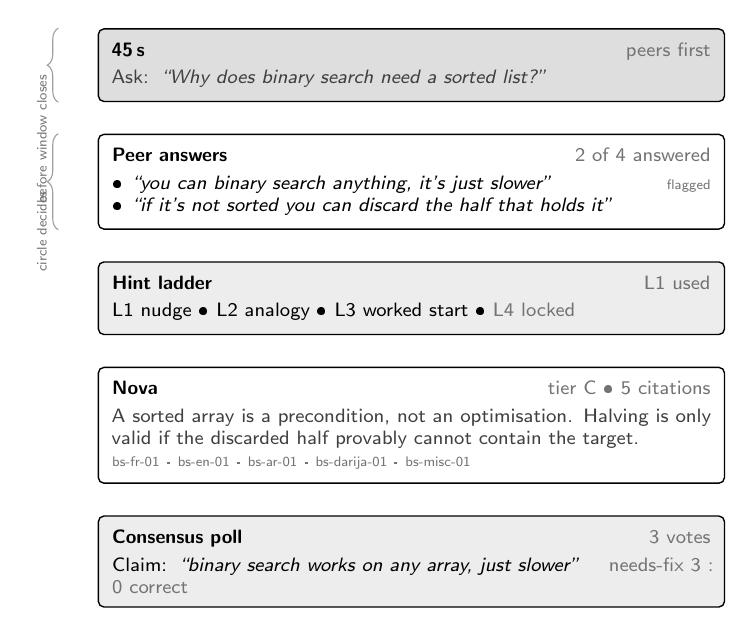
\begin{tikzpicture}[
  font=\sffamily\scriptsize,
  blk/.style={draw=ink0,fill=white,rounded corners=2pt,align=left,inner sep=5pt,
              text width=7.6cm,line width=0.5pt},
  blkf/.style={blk,fill=fillA},
  blkd/.style={blk,fill=fillB},
  tag/.style={font=\sffamily\tiny,color=ink2},
]
\node[blkd] (count) {\textbf{45\,s} \hfill{\color{ink2}peers first}\\[2pt]
  {\color{ink1}Ask: \emph{``Why does binary search need a sorted list?''}}};
\node[blk,below=4mm of count] (peers) {\textbf{Peer answers} \hfill{\color{ink2}2 of 4 answered}\\[2pt]
  \textbullet\ \emph{``you can binary search anything, it's just slower''}
    \hfill{\color{ink2}\tiny flagged}\\
  \textbullet\ \emph{``if it's not sorted you can discard the half that holds it''}};
\node[blkf,below=4mm of peers] (ladder) {\textbf{Hint ladder} \hfill{\color{ink2}L1 used}\\[2pt]
  L1 nudge \textbullet\ L2 analogy \textbullet\ L3 worked start \textbullet\
  {\color{ink2}L4 locked}};
\node[blk,below=4mm of ladder] (nova) {\textbf{Nova} \hfill{\color{ink2}tier C \textbullet\ 5 citations}\\[2pt]
  {\color{ink1}A sorted array is a precondition, not an optimisation. Halving is only
  valid if the discarded half provably cannot contain the target.}\\
  {\color{ink2}\tiny bs-fr-01 · bs-en-01 · bs-ar-01 · bs-darija-01 · bs-misc-01}};
\node[blkf,below=4mm of nova] (poll) {\textbf{Consensus poll} \hfill{\color{ink2}3 votes}\\[2pt]
  Claim: \emph{``binary search works on any array, just slower''} \hfill
  {\color{ink2}needs-fix 3 : 0 correct}};
\draw[decorate,decoration={brace,amplitude=4pt,mirror},ink3]
  ($(count.north west)+(-0.5,0)$) -- ($(count.south west)+(-0.5,0)$)
  node[midway,left=6pt,rotate=90,font=\sffamily\tiny,color=ink2]{before window closes};
\draw[decorate,decoration={brace,amplitude=4pt,mirror},ink3]
  ($(peers.north west)+(-0.5,0)$) -- ($(peers.south west)+(-0.5,0)$)
  node[midway,left=6pt,rotate=90,font=\sffamily\tiny,color=ink2]{circle decides};
\end{tikzpicture}
\caption{The session room, in reading order. The countdown is the hero; peers occupy the
space between asking and knowing; the ladder is offered before the answer; citations sit
under the answer rather than beside it.}
\label{fig:session}
\end{figure}

\subsection{Countdown as a contract}

The countdown is not decoration. It is the visible half of the server-authoritative window:
the client derives the remaining time from \code{windowEndsAt}, renders it, and disables the
peer-answer affordance at zero. Because the deadline lives on the server, a slow clock or a
backgrounded tab cannot extend the window, and the UI cannot accidentally promise time the
server will not grant.

\subsection{Staged progress instead of fake streaming}

Responses arrive whole. The interface therefore shows the pipeline stages
(\emph{retrieving}, \emph{checking similar}, \emph{writing}, \emph{verifying}) as an ordered
stepper with completed steps marked, and never renders a partial answer that the server has
not sent. This is a deliberate honesty choice: a token-by-token animation over a whole
response would be theatre, and the first time it desynchronised from the data it would read
as a bug.

\subsection{The zero-model skeleton}

The first paint of any AI-bearing section is a skeleton that requires no model call. It
renders in under 200\,ms, which is the number in \code{config/router.yaml}, and it is the
reason the screen never shows an empty box while the queue drains. The skeleton is shaped
like the content it will hold, so the transition does not reflow the page.

\section{Design system}

The interface is built from tokens rather than from components with hardcoded values, so
that a change to spacing or type propagates rather than being hunted.

\begin{table}[htbp]
\centering
\caption{Design tokens and the constraint each encodes.}
\label{tab:tokens}
\footnotesize
\begin{tabularx}{\textwidth}{@{}p{3.1cm}X@{}}
\toprule
\textbf{Token group} & \textbf{Rule, and why} \\
\midrule
Type & A single family with a display weight for headings and a text weight for body.
  Optical sizing and tracking are set per size, because a heading tracked for 14\,pt reads
  loose at 32\,pt \\
Space & A 4\,pt base scale. Every margin and padding is a multiple, so vertical rhythm
  holds across screens written by different people \\
Colour & A restrained ink scale plus one accent per context mode. Contrast is asserted
  against WCAG AA in a test, not eyeballed \\
Motion & Durations and easings are tokens; every transition respects
  \code{prefers-reduced-motion} through a single hook \\
Radius and rule & One radius for controls, one for cards, one hairline weight. The
  restraint is what makes dense screens readable \\
Touch & 44\,px minimum target, asserted by a sizing test rather than assumed from padding \\
\bottomrule
\end{tabularx}
\end{table}

\paragraph{No-shame styling.} A design rule with ethical content: a low S-B-U tier is
rendered as a gentle pulse, never as red, and a wrong answer is met with a guiding question
rather than a reprimand. This is implemented at the token level --- there is no ``error red''
in the palette for learner-facing surfaces --- so a future contributor cannot introduce
shame styling without changing the design system.

\paragraph{Anonymous by default where it matters.} Questions can be posted anonymously, and
``me too'' is a private signal between the learner and the coach rather than a public
confession. Both exist because the social cost of asking the simple question is the
specific failure the product is designed to remove.

\section{Internationalization and right-to-left}
\label{sec:i18n}

The interface ships 357 translated keys across four registers: Arabic, Tunisian Darija,
French and English. Three properties were required and are enforced.

\begin{enumerate}[leftmargin=1.6em,itemsep=2pt]
  \item \textbf{Parity.} A checker script walks the key table and fails the build if any key
        is missing a translation in any language, so no screen can fall back to English
        mid-flow.
  \item \textbf{Direction.} Arabic and Darija are right-to-left. Layout uses logical
        properties rather than left/right, so the mirror is a document-level attribute
        change rather than a second stylesheet.
  \item \textbf{Darija is a first-class register, not a translation of Arabic.} The Darija
        strings are written in Darija, including Arabizi-tolerant phrasing where the
        product speaks in that register, and the tests treat Darija as a required locale
        rather than an optional one.
\end{enumerate}

The i18n test also asserts that no user-visible string is hardcoded in a component ---
a rule that is easy to state and easy to break under deadline, which is exactly why it is
a test.

\section{Accessibility}

Accessibility is treated as a set of gates rather than a checklist. The gates that run on
every build are:

\begin{itemize}[leftmargin=1.4em,itemsep=2pt]
  \item \textbf{axe-core on rendered screens}, including the 404 and the crash card. The
        gate runs the real engine against the real DOM rather than asserting hand-counted
        attributes, so a component that loses its label fails.
  \item \textbf{Keyboard completeness}: every interactive element is reachable and
        operable, and focus is visible. A focus trap in a sheet is tested rather than
        trusted.
  \item \textbf{Announced route transitions}: the lazy-chunk fallback carries a status role
        and a label in the learner's own language, so a screen reader announces
        ``loading'' in Arabic rather than in English.
  \item \textbf{Reduced motion}: one hook owns the media query, so no component can opt out
        of it by accident.
\end{itemize}

\begin{note}[Why the crash card is tested for accessibility]
The screen a user sees when something breaks is the screen they see at their most
confused. It is also the screen most likely to be written in a hurry. Testing it for
contrast, focus and labels catches the class of bug that only appears in the worst
moment.
\end{note}

\section{Offline behaviour}

The service worker precaches the application shell and the offline pack, so a dropped
connection does not present a browser error page. In the \code{BLACK} degradation state the
client serves the pack locally with an explicit \code{offline:true} label, which is the
honest version of the promise: the learner knows the answer came from a snapshot rather
than from the model. Writes that arrive while offline are queued and synced later, and the
session continues with peer work, polls, role-play and flashcards --- the activities that
never needed the model in the first place.

\section{Performance}

The performance budget is small and stated: a skeleton in under 200\,ms, first paint from
the precached shell on a repeat visit, and no model call on the critical path of a route
transition. Route-level code splitting keeps the initial bundle to the landing page plus the
shell; the session room, which is the heaviest screen, is fetched only when a learner enters
a circle.

\chapter{Privacy and Ethics}
\label{ch:privacy}

The challenge asks for a companion usable by learners, which in practice means learners who
may be minors, in groups, on shared devices. This chapter describes privacy as a set of
enforced properties rather than a policy statement, because a policy statement cannot be
tested and therefore cannot be relied on.

\section{The schema gate}
\label{sec:privacy-gate}

The central claim is narrow and checkable: the persona collection has no column in which a
name, a photograph, a gender or a region could be stored. Not that such data is unused ---
that there is nowhere to put it. The claim is maintained by a test that reads the schema
sources and fails the build if a forbidden field name appears.

\begin{lstlisting}[language=Java,caption={The build gate. It reads the schema sources, strip the explanatory comment that names the forbidden fields, and asserts nothing else mentions them.}]
const FORBIDDEN = /\bgender\b|\bsex\b|\bregion\b|\bcountry\b|\bphoto\b|\bbirth\b|\bage\b|\baddress\b|\bphone\b|\bemail\b/i;

it('no schema source contains a forbidden field name', () => { /* ... */ });
it('no bare `name` prop exists anywhere (only `nickname`)', () => { /* ... */ });
\end{lstlisting}

The second assertion is the interesting one. \code{name} is such a natural field name that
it reappears by reflex, so the gate allows the substring only inside \code{nickname} and
\code{username}. A learner is therefore always an artificial identifier ---
\code{L-01}, \code{L-02} --- with a nickname and a neutral avatar key chosen from a fixed
set. There is no field in which a real name would fit, so the guarantee does not depend on
anyone remembering it.

\section{PII screening before model calls}

Text that reaches the model is screened first, at every write boundary, by a pure function
that returns both the cleaned text and the kinds of finding it removed.

\begin{table}[htbp]
\centering
\caption{The PII screen. Each pattern runs before any string leaves the process.}
\label{tab:pii}
\footnotesize
\begin{tabularx}{\textwidth}{@{}p{2.5cm}p{4.0cm}X@{}}
\toprule
\textbf{Kind} & \textbf{Pattern} & \textbf{Redaction} \\
\midrule
\code{email} & Address-shaped token & \code{[email]} \\
\code{phone} & Phone-shaped digit run with separators, including international prefixes
             & \code{[phone]} \\
\code{address\_hint} & Street-number patterns in French, Arabic and Tunisian usage
             & \code{[address]} \\
\code{id\_digits} & Any run of eight or more digits & \code{[id]} \\
\bottomrule
\end{tabularx}
\end{table}

Returning findings rather than a boolean is a product decision: the learner can be told
\emph{what} was removed, which converts a silent mutation into an explicit one. It also
lets the interface advise against pasting a phone number rather than silently swallowing
it.

\section{Data minimisation in the model payload}

What is sent to the provider is public course material and the learner's own message,
screened. Nothing else. There is no profile, no history replay and no analytics payload in
a model call, which is the concrete meaning of data minimisation here. The knowledge base is
team-written and synthetic, so a grounded request contains no third-party text either ---
which sidesteps a licensing question as well as a privacy one.

\section{Logs and retention}

Logs pass through a scrubber, and telemetry has a ninety-day TTL enforced by a database
index rather than a scheduled job. The distinction matters: a retention policy implemented
by a cron job is satisfied only if the job runs, whereas a TTL index is satisfied by
construction. Deletion follows the same principle, with a thirty-day grace window and a
tombstone afterwards (\S\ref{sec:datasubject}).

\section{Ethics of the interaction}

Three ethical positions are encoded in behaviour rather than stated in a document.

\paragraph{No public ranking.} There is deliberately no leaderboard. A circle shows its
S-B-U rings --- participation balance, help quality and verified agreement --- and never a
ranking of people. The blueprint states this as a constraint on the frontend, and the
constraint is structural: no leaderboard component exists.

\paragraph{Wrong answers are met with a question.} The register guides for all four
languages carry an explicit no-shaming rule, and the design system has no learner-facing
error red. A wrong answer is the most informative moment in a session, and treating it as a
fault trains learners to hide it.

\paragraph{Participation equity is visible to facilitators, not to peers.} A facilitator
sees the \emph{Share} ring and can route attention to a quiet learner. The learner
themselves never sees a public score, and the coach nudge is private. The design exposes
inequity to the person who can act on it and to nobody else.

\section{Security posture as a privacy control}

The two are connected: a bearer token in \code{sessionStorage} means an XSS is session
theft, which is a privacy incident rather than a cosmetic bug. This is why the CSP is built
by a testable function with \code{script-src 'self'} and no inline script, and why the
default-deny guard matters beyond access control --- it limits the blast radius of a stolen
token to the routes that token's role may reach.

\begin{keyfinding}[What can be asserted to the jury]
There is no column for a name, photo, gender or region, and a build gate fails if one
appears. PII is screened before any model call, and the screen reports what it removed.
Retention is enforced by the database. Deletion has a reversible grace window and a
tombstone afterwards. There is no leaderboard, and there is no learner-facing error red.
\end{keyfinding}

\chapter{Testing Strategy and Results}
\label{ch:testing}

The system makes strong claims --- that privacy is structural, that the provider is
isolated, that the ladder cannot be short-circuited, that larger-model usage is a
minority. A claim without a gate is an aspiration, so each of these is a test whose name
states the guarantee.

\section{The pyramid, and where it is deliberately unusual}

\begin{figure}[htbp]
\centering
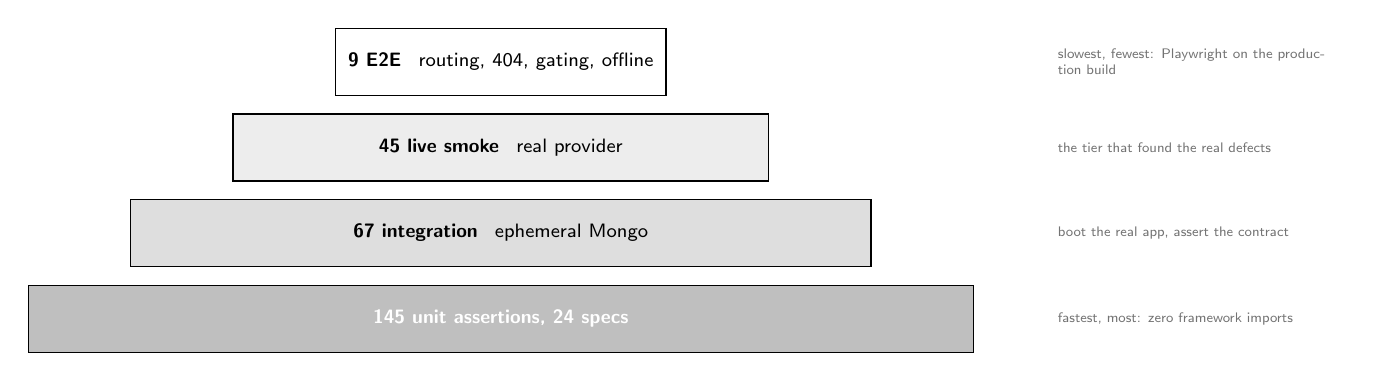
\begin{tikzpicture}[
  font=\sffamily\scriptsize,
  lay/.style={draw=ink0,align=center,line width=0.5pt,minimum height=8.5mm},
  l1/.style={lay,fill=white,minimum width=4.2cm},
  l2/.style={lay,fill=fillA,minimum width=6.8cm},
  l3/.style={lay,fill=fillB,minimum width=9.4cm},
  l4/.style={lay,fill=fillC,minimum width=12.0cm,text=white},
  side/.style={font=\sffamily\tiny,color=ink2,align=left,anchor=west,
               text width=3.55cm},
]
\node[l1] (e2e) {\textbf{9 E2E} \enspace routing, 404, gating, offline};
\node[l2,below=2.2mm of e2e] (live) {\textbf{45 live smoke} \enspace real provider};
\node[l3,below=2.2mm of live] (int) {\textbf{67 integration} \enspace ephemeral Mongo};
\node[l4,below=2.2mm of int] (unit) {\textbf{145 unit assertions, 24 specs}};
\node[side] at (6.95,0|-{e2e.center}) {slowest, fewest: Playwright on the production build};
\node[side] at (6.95,0|-{live.center}) {the tier that found the real defects};
\node[side] at (6.95,0|-{int.center}) {boot the real app, assert the contract};
\node[side] at (6.95,0|-{unit.center}) {fastest, most: zero framework imports};
\end{tikzpicture}
\caption{Test tiers. The unusual width is deliberate: this project invested far more in
unit and integration assertions than in E2E, because the guarantees it claims are
properties of pure functions and of the API contract rather than of user journeys.}
\label{fig:pyramid}
\end{figure}

\section{Tier 1: pure-domain unit tests}

Twenty-four spec files, 145 assertions, zero Nest imports. These run without a database or
a container, so they run on every keystroke in development and on every push in CI. They
cover exactly the logic that a refactor could silently break:

\begin{table}[htbp]
\centering
\caption{Representative unit specs and the guarantee each one holds.}
\label{tab:units}
\footnotesize
\begin{tabularx}{\textwidth}{@{}p{3.7cm}X@{}}
\toprule
\textbf{Spec} & \textbf{Guarantee} \\
\midrule
\code{schema-gate} & No forbidden field appears in any schema, and no bare \code{name}
  prop exists anywhere \\
\code{adapter-isolation} & Only \code{src/ai} imports the provider adapter; only the
  adapter and the validated config read model environment keys \\
\code{cache-key} & Equivalent re-asks collapse: normalisation, sorted chunk ids, ladder
  state \\
\code{credits-math} & The log cap holds the worked example (12 plain $\approx 5.1$ versus
  $7$), and dispersion is a coefficient of variation \\
\code{sbu-math} & The three rings, the display thresholds and the \code{needs\_human}
  predicate \\
\code{router-pure} & A malformed Pulse reply degrades one turn rather than failing; at
  most one pulse per window \\
\code{degradation-provider} & A provider 429 or timeout maps to the correct state, and
  recovery maps back \\
\code{tokens}, \code{credentials}, \code{token-guard} & HMAC round-trip, epoch revocation,
  scrypt verification, previous-secret rotation \\
\code{csp} & The CSP asserts \code{script-src 'self'} and no inline script \\
\code{pii}, \code{scrubber} & Each pattern is caught, and the finding is reported \\
\code{user-messages} & Every domain error has all four localized messages \\
\code{circle-budget} & The per-circle daily ceiling is the binding limit, not the
  per-session cap \\
\code{seed-kb} & The seed files and the manifest agree in both directions \\
\bottomrule
\end{tabularx}
\end{table}

\section{Tier 2: integration tests}

Nine specs, 67 assertions, booting the real Nest application against an ephemeral MongoDB.
This tier exists to test the things that only a running app can get wrong: the error
contract, the authorization matrix, session-end idempotency, and retention.

\begin{table}[htbp]
\centering
\caption{Integration specs and the behaviour they pin down.}
\label{tab:integr}
\footnotesize
\begin{tabularx}{\textwidth}{@{}p{3.7cm}X@{}}
\toprule
\textbf{Spec} & \textbf{Behaviour} \\
\midrule
\code{foundation} & App boots, health and readiness, uniform 404 and 400 shapes \\
\code{authz-matrix} & Learner $\times$ mentor $\times$ admin $\times$ anonymous
  $\times$ cross-circle: every cell asserted, including denials \\
\code{accounts} & Upgrade path keeps progress; epoch bump signs out other devices;
  export excludes the reusable secret \\
\code{cfas-slice} & The full ask flow with a stubbed model: peers answer / nobody
  answers / skip, each settled correctly \\
\code{ai-platform} & Governor, queue, cache and degradation wired together; quota
  exhaustion downgrades rather than fails \\
\code{deterministic-core} & Retrieval, matcher and cache are reproducible across runs \\
\code{phase5-outputs} & Capsule, quiz, whisper, mentor and board outputs respect their
  limits \\
\code{rate-limit} & Named budgets reject past their limit and the rejection is shaped
  correctly \\
\code{retention} & Deletion schedules the purge, restore reverses it, purge tombstones the
  identifier \\
\bottomrule
\end{tabularx}
\end{table}

Two of these deserve emphasis because they encode decisions rather than behaviour.

\paragraph{The authorization matrix is a table, not a story.} Twelve assertions walk every
combination of actor and resource, including cross-circle access. A row that is denied is
asserted to be denied, so a future ``convenience'' relaxation of a check fails a named
test.

\paragraph{Session-end is asserted idempotent.} The debrief screen remounts, and the first
version of the code credited the session twice when it did. That is now a test, and the fix
is described as what it was: a defect found by a remount, not by review.

\section{Tier 3: the live smoke}
\label{sec:smoke}

The most informative tier is a 45-check smoke that boots the API against the \emph{real}
inference platform and walks every endpoint in dependency order. It is not a unit test with
a mock: it spends real model calls, so it measures the routing policy rather than
simulating it.

\begin{table}[htbp]
\centering
\caption{The live smoke in collapse order. Each group depends on the one above it, so a
failure localises rather than cascading.}
\label{tab:smoke}
\footnotesize
\begin{tabularx}{\textwidth}{@{}p{1.2cm}p{4.6cm}X@{}}
\toprule
\textbf{\#} & \textbf{Group} & \textbf{Representative checks} \\
\midrule
1--4 & Platform & \code{/healthz}; readiness with Mongo connected; KB at least 39 chunks with
  claims; degradation green at boot \\
5--11 & Identity & Session issues an HMAC token; \code{/me} has no passport before DNA;
  the four items are exactly L1 S1 G1 C1; completion writes a passport; a bad level is
  rejected with the uniform 400; the explain card renders from the passport \\
12--18 & Circles & Create returns a join code and a host token; a second learner joins;
  duplicate nickname is 409; the member list is correct; the context config has an agenda;
  session start is ledger-backed \\
19--26 & Circle-First Ask & Question opens with a window and a real compact pulse; Quick
  Take prepared by a real call; the peer view hides the asker and serves a stable ETag;
  peer answer awards credits and the Auditor verifies with a real call; skip resolves at
  tier C with citations; L1 is T0 and L4 is refused before L1--L3; a seeded misconception
  goes poll-first \\
27--33 & Outputs & ``Me too'' emits an event; session credits are correct; the capsule is
  three bullets within the word cap; a quiz battle yields XP; Whisper returns all four
  drift categories; a mentor joins as observer, notes and gets a brief; the matcher is
  deterministic and the board lists circles \\
34--40 & Facilitation & Coach card and a rephrased nudge within the token cap; game caps
  hold and there is no leaderboard; the dashboard is aggregate-only; circle health exposes
  S/B/U and \code{needsHuman}; telemetry is readable; solo runs two turns and a hat with
  zero L calls \\
41--45 & Operations & \code{/metrics} has all report keys; chaos forces orange and flips
  back; session end is idempotent; Whisper rejects a one-link chain; domain errors are
  localized for all four registers; unknown route and validation failure return uniform
  shapes \\
\bottomrule
\end{tabularx}
\end{table}

\begin{keyfinding}[Live smoke result]
\textbf{45 passed, 0 failed} against the real inference platform. Tier split during the run:
\textbf{C = 13, L = 2}, giving \code{lShare = 0.133} --- roughly half the $<0.25$ ceiling.
Cache hits are metered rather than inferred, and \code{/metrics} is asserted to contain every
key the report cites.
\end{keyfinding}

\section{Tier 4: gates}

Three gates run in CI before any test, because they are cheap and their failures are the
most expensive to discover late.

\begin{description}[leftmargin=0pt,style=nextline,itemsep=2pt]
  \item[Secrets scan] Runs first. Fails on credentials, keys or \code{.env} content in the
    repository.
  \item[Schema gate] Fails if a forbidden persona field appears (\S\ref{sec:privacy-gate}).
  \item[Clean clone] A job that installs and builds the frontend from tracked files only.
    It exists because a clean clone once failed to compile when a route directory was
    untracked, and a green local build had hidden it.
\end{description}

\section{Tier 5: evaluation fixtures}

Beyond unit and integration tests, five replayable evaluation sets measure quality rather
than correctness, and \code{npm run eval:all} emits reportable metrics from all of them:

\begin{table}[htbp]
\centering
\caption{Evaluation fixtures. These measure precision and parity, which no assertion can.}
\label{tab:evals}
\footnotesize
\begin{tabular}{@{}p{3.9cm}rp{5.7cm}@{}}
\toprule
\textbf{Fixture} & \textbf{Size} & \textbf{What it measures} \\
\midrule
\code{confusion\_set.jsonl} & 20 & Precision at detecting learner confusion signals \\
\code{lang\_parity.jsonl} & 24 & Parity across all four registers, scored for human
  quality \\
\code{seeded\_errors.jsonl} & 3 & Whether a seeded misconception is actually caught \\
\code{whisper\_groundtruth} & 2 & Drift-map agreement against a reference \\
\code{users\_fixtures.json} & 4 & A reproducible roster for the demo and the smoke \\
\bottomrule
\end{tabular}
\end{table}

\section{Load and SLO}

The peer window implies polling, which is the one place where a modest client count can
still produce real load. A dedicated load script drives the \code{/state} route and treats
the service-level objective as a pass/fail gate rather than as a graph to look at: p95 must
stay under 50\,ms, and the script exits non-zero if it does not. Making an SLO a build gate
is the difference between a target and a requirement.

\section{What testing found}

Listing defects found by tests is more useful to a jury than listing the tests themselves,
because it shows the strategy was load-bearing.

\begin{table}[htbp]
\centering
\caption{Representative defects caught by each tier.}
\label{tab:defects}
\footnotesize
\begin{tabularx}{\textwidth}{@{}p{2.5cm}X@{}}
\toprule
\textbf{Tier} & \textbf{Defect} \\
\midrule
Live smoke & Learners were refused on the very circle-health poller they depend on --- an
  authorization ordering bug that no unit test could see \\
Live smoke & 429 from the provider hard-failed the whole suite, so the same code flapped
  between green and red; now one bounded retry honouring \code{Retry-After} \\
Integration & Session end credited twice when the debrief screen remounted; fixed and
  asserted idempotent \\
Integration & A DNS answer on the DNA screen exposed display strings while the API
  validated enum values, so the screen could never submit \\
Unit & A classroom-scale loop could exceed the per-session cap by an order of magnitude;
  the per-circle daily ceiling now bounds it \\
Clean clone & The build failed from a clean checkout because a route directory was
  untracked; a dedicated CI job now makes that unmergeable \\
\bottomrule
\end{tabularx}
\end{table}

\section{Reproduction}

The appendix states the exact procedure (\S\ref{app:repro}). The short version is five
steps for the API and four for the web client, both from a clean checkout, with
\code{npm run test:unit}, \code{test:int}, \code{test:schema} and \code{lint:secrets} as
the gates, and \code{npm run smoke:live} as the end-to-end verification that requires
provider credentials.

\chapter{Results and Discussion}
\label{ch:results}

This chapter reports what was measured, and then argues about what the measurements do and
do not support. Separating the two is the point: a final report that presents a live
smoke as evidence of learning efficacy would be making a claim the data cannot carry.

\section{Delivered system}

\begin{table}[htbp]
\centering
\caption{Delivered system by the numbers. Every figure in this table is checkable from the
repository.}
\label{tab:numbers}
\footnotesize
\begin{tabularx}{\textwidth}{@{}p{5.2cm}p{2.3cm}X@{}}
\toprule
\textbf{Dimension} & \textbf{Count} & \textbf{Where} \\
\midrule
Backend source & 9{,}603 lines & \code{halqa-api/src} \\
Frontend source & 8{,}371 lines & \code{halqa-web/src} \\
Domain modules, zero framework imports & 15 & \code{src/domain} \\
Feature modules & 25 & \code{src/modules} \\
Controllers / HTTP routes & 20 / 68 & under \code{/api/v1} \\
MongoDB collections / indexes & 18 / 22 & \code{src/persistence} \\
Migrations (idempotent) & 2 & XP backfill, deletion fields \\
Frontend routes & 15 & 13 authenticated, 1 dev-only \\
Translated interface keys & 357 & four registers, parity-gated \\
Knowledge-base chunks & 39 & two packs, manifest-verified \\
Offline-pack snippets & 30 & served in RED and BLACK \\
Unit assertions / spec files & 145 / 24 & pure domain \\
Integration assertions / spec files & 67 / 9 & ephemeral Mongo \\
E2E tests & 9 & production build, Playwright \\
Live smoke checks & 45 & real inference platform \\
Evaluation fixtures & 53 cases & five replayable sets \\
\bottomrule
\end{tabularx}
\end{table}

\section{The routing policy, measured}
\label{sec:metrics-live}

The headline quantitative result is the tier split. It is reported as a share of
\emph{calls}, not as a share of tokens or of time, because the constraint being managed is
quota rather than latency.

\begin{figure}[htbp]
\centering
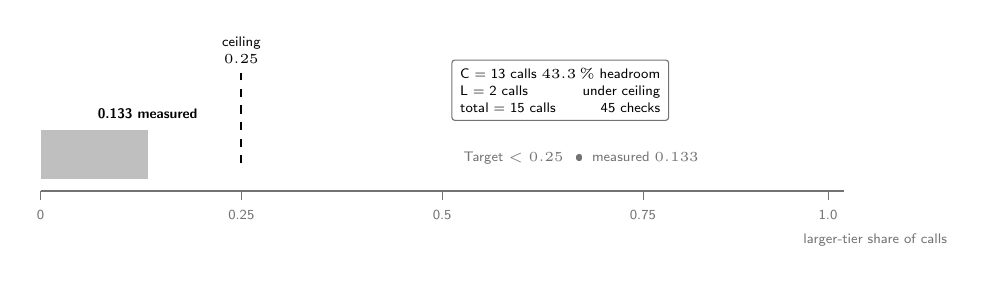
\begin{tikzpicture}[
  font=\sffamily\scriptsize,
  bar/.style={draw=ink0,line width=0.5pt},
  ax/.style={draw=ink2,line width=0.4pt},
]
% axis
\draw[ax] (0,0) -- (10.2,0);
\foreach \x/\v in {0/0, 2.55/0.25, 5.1/0.5, 7.65/0.75, 10/1.0}{
  \draw[ink2,line width=0.3pt] (\x,0) -- (\x,-0.12);
  \node[font=\sffamily\tiny,color=ink2,below] at (\x,-0.12) {\v};
}
\node[font=\sffamily\tiny,color=ink2,below] at (10.6,-0.42) {larger-tier share of calls};
% target line
\draw[ink0,dashed,line width=0.7pt] (2.55,0.35) -- (2.55,1.5);
\node[font=\sffamily\tiny,color=ink0,above,align=center] at (2.55,1.5) {ceiling\\ $0.25$};
% measured
\fill[fillC] (0,0.15) rectangle (1.36,0.78);
\node[font=\sffamily\tiny,color=ink0,above] at (1.36,0.80) {\textbf{0.133 measured}};
% breakdown annotation
\node[draw=ink2,fill=white,rounded corners=1pt,inner sep=3pt,align=left,
      font=\sffamily\tiny] at (6.6,1.28)
  {C = 13 calls \hfill $43.3\,\%$ headroom\\ L = 2 calls \hfill under ceiling\\
   total = 15 calls \hfill 45 checks};
\node[font=\sffamily\tiny,color=ink2,align=left,anchor=north west] at (5.25,0.62)
  {Target $<0.25$ \enspace\textbullet\enspace measured $0.133$};
\end{tikzpicture}
\caption{Measured tier split from the live smoke. The measured share sits at roughly half
the permitted ceiling, which is the result the routing policy was designed to produce: the
larger tier is used, but it must earn each call.}
\label{fig:lshare}
\end{figure}

Read this graph carefully, because it is easy to over-read. A low share is only good if
quality does not collapse, and this measurement does not establish that the compact tier
was \emph{sufficient} for the tasks it handled --- it establishes that the escalation gate
did not admit them. The evidence for sufficiency is the eval set and the rubric review,
not the share itself.

\section{Latency budgets}

The latency figures below are \emph{budgets in configuration} that the system enforces,
plus the one latency SLO that is a build gate. They should be distinguished from the smoke
run's own durations, which are dominated by the provider's variable speed and are not
reported as a performance claim.

\begin{table}[htbp]
\centering
\caption{Latency budgets and how each is enforced.}
\label{tab:latency}
\footnotesize
\begin{tabularx}{\textwidth}{@{}p{3.6cm}p{2.1cm}X@{}}
\toprule
\textbf{Path} & \textbf{Budget} & \textbf{Enforcement} \\
\midrule
Skeleton, zero model calls & $<200$\,ms & \code{skeleton\_ms}; asserted in budget tests \\
Compact completion & $<4$\,s & \code{c\_complete\_ms}; p50/p95 on \code{/metrics} \\
Larger completion & $<12$\,s & \code{l\_complete\_ms}; p50/p95 on \code{/metrics} \\
Peer state poll, p95 & $<50$\,ms & \code{load:poller} treats the SLO as pass/fail \\
\bottomrule
\end{tabularx}
\end{table}

\section{Functional verification}

Each objective from \S\ref{ch:intro} is closed below by pointing at the artefact rather
than at an intention.

\begin{table}[htbp]
\centering
\caption{Objectives closed.}
\label{tab:objectives-closed}
\footnotesize
\begin{tabularx}{\textwidth}{@{}p{0.7cm}X p{4.6cm}@{}}
\toprule
\textbf{\#} & \textbf{Closing evidence} & \textbf{Residual limitation} \\
\midrule
O1 & Timed window with dual settlement, peer-first rate metered; smoke group 19--26
   & Peer-first \emph{rate} is measured, not yet compared to a control group \\
O2 & Auditor with checklist-first path and poll-first fallback; seeded-misconception check
   in both the smoke and the eval set & Three seeded errors is a small set \\
O3 & DNA passport writes level, style, register and eagerness; bandit updates from check
   outcomes; language parity across four registers & Bandit step sizes are configured, not
   tuned on real learners \\
O4 & \code{lShare = 0.133} from the call ledger, under the $0.25$ ceiling & One run of 15
   calls; a longer run would tighten the interval \\
O5 & Four-state machine, chaos-tested; 30-snippet offline pack served in BLACK & Offline
   pack covers two topics \\
O6 & Schema gate, PII screen before every call, retention by TTL, export and deletion
   & Consent capture is out of scope for this submission \\
\bottomrule
\end{tabularx}
\end{table}

\section{Discussion: what the numbers mean}

\paragraph{The tier split is a process result, not an accuracy result.} It shows that the
escalation gate is conservative in practice and that the compact tier absorbed the routine
work. It does not show that a larger model would not have produced better answers --- that
comparison requires an evaluation of answer quality across tiers, which is what the
language-parity and confusion sets are for.

\paragraph{The smoke is a contract test at full depth.} Forty-five checks across the
dependency order of the product is unusually thorough for a hackathon submission, and it is
where most defects were found. But it runs a single synthetic journey, so it exercises
breadth rather than depth of behaviour.

\paragraph{Forty-five checks is not forty-five users.} This distinction is the most
important one in the report. Nothing here establishes that peer-first orchestration improves
learning outcomes. It establishes that the mechanism is implemented, coherent, measured and
not obviously broken --- which is the correct claim for this submission, and the weaker
claim is the only one the evidence supports.

\section{Threats to validity}
\label{sec:threats}

\begin{table}[htbp]
\centering
\caption{Threats to validity, and how each is mitigated or honestly bounded.}
\label{tab:threats}
\footnotesize
\begin{tabularx}{\textwidth}{@{}p{3.0cm}X@{}}
\toprule
\textbf{Threat} & \textbf{Assessment} \\
\midrule
Small call volume & Fifteen model calls in the smoke give a coarse estimate of the share.
  Mitigation: the share is computed from a persisted ledger, so it can be recomputed
  over any window, including a rehearsal with real cohorts \\
Synthetic knowledge base & Two topics and 39 chunks do not represent a curriculum.
  Mitigation: the pack format is the extension point --- adding a course is a JSON file
  plus a manifest row, and the manifest gate prevents an inconsistent pack from shipping \\
Single provider & The routing policy is measured on one platform. Mitigation: all provider
  knowledge is in one adapter, so the same smoke can be re-run against another provider or
  a self-hosted model with no feature change \\
No longitudinal learning data & The bandit and the S-B-U rings are configured from
  pedagogy rather than fitted to observed learners. This is a genuine limitation, stated
  as such \\
Demo rehearsed, not fielded & The four-language demo path is rehearsed end to end, but
  real-user testing in two contexts is planned for the post-submission rehearsal and is not
  claimed as a result here \\
Clock and network assumptions & Server-authoritative windows remove the client-clock
  dependency; the offline pack removes the connectivity dependency; shared-device sessions
  remain a usability risk that only real cohorts can measure \\
\bottomrule
\end{tabularx}
\end{table}

\section{Comparison with a conventional assistant}

\begin{table}[htbp]
\centering
\caption{How the design differs from the obvious alternative, stated as trade-offs rather
than as superiority claims.}
\label{tab:compare}
\footnotesize
\begin{tabularx}{\textwidth}{@{}p{3.2cm}X X@{}}
\toprule
& \textbf{Conventional assistant} & \textbf{HALQA} \\
\midrule
Who answers first & The model & Peers, inside a timed window \\
Cost profile & Every turn is a model call & Templates and cache first; a call must be
  justified \\
Failure mode & Screen waits or errors & Four declared states with changed promises \\
Personalization & Prompt-level, per session & Passport plus a bandit that persists \\
Privacy & Policy text & Schema gate that fails the build \\
Facilitation & Not addressed & S-B-U rings and \code{needs\_human} routing \\
Weakness & Fast, broad, forgettable & Slower to first answer; needs a group to be at its
  best, which is why solo mode reuses the same ladder \\
\bottomrule
\end{tabularx}
\end{table}

\chapter{Business Model}
\label{ch:business}

The challenge requires a business-model note, and the honest version of one for the final
report is not a revenue projection. It is an answer to three questions: who has this
problem badly enough to change behaviour, what exactly they receive, and how the thing pays
for itself and survives its provider.

\section{Target users}

\begin{table}[htbp]
\centering
\caption{Three segments, and the reason each one is reachable without a sales team.}
\label{tab:segments}
\footnotesize
\begin{tabularx}{\textwidth}{@{}p{2.9cm}X p{4.2cm}@{}}
\toprule
\textbf{Segment} & \textbf{Why they feel the problem} & \textbf{Entry point} \\
\midrule
University tutoring and revision circles & Small groups already meet; the failure is
  coordination, and nobody is paid to fix it & IEEE student branches and campus clubs \\
Training centres and bootcamps & Mixed-level cohorts where one learner dominates and the
  trainer cannot watch every group & The facilitator board is the trainer's tool \\
Self-learning communities & Motivated learners with no facilitator at all; they need
  structure more than content & Public circles, join by code or QR \\
\bottomrule
\end{tabularx}
\end{table}

The three segments share a property that makes adoption plausible: the product enters an
existing ritual rather than asking for a new one. A revision circle already meets; HALQA
changes how the meeting runs, not whether it happens.

\section{Value proposition}

The proposition is stated in terms its buyer can check.

\begin{itemize}[leftmargin=1.4em,itemsep=2pt]
  \item \textbf{Fair turns without extra facilitation.} The window and the \emph{Share}
        ring make participation visible, so a group can correct itself without an adult in
        the room.
  \item \textbf{Fewer wrong answers spreading.} The Auditor and poll-first behaviour
        intervene before a misconception becomes consensus, which is the expensive failure
        in peer learning.
  \item \textbf{Memory of the session.} The revision capsule and the quiz bank turn a
        conversation into something revisable, at no extra effort.
  \item \textbf{Bounded cost.} Token spend is a documented policy with a measured ceiling,
        so the cost of a session is predictable rather than proportional to enthusiasm.
  \item \textbf{Visibility for the person responsible.} The board shows which circle needs a
        human, which is the only feature a training centre will pay for.
\end{itemize}

\section{Adoption path}

\paragraph{Step 1 --- bottom-up pilot.} IEEE student branches and campus clubs already in
the WIE ACT network run HALQA for one revision cycle. The two things learned from a pilot
are not usage statistics but \emph{pack demand}: which course the cohort actually revises.
That feeds the seed knowledge base, which is the real asset.

\paragraph{Step 2 --- department licensing.} Tutoring programmes buy per-cohort access, and
the board view is the stakeholder-facing artefact. A department does not buy a chatbot; it
buys evidence that its tutoring hours are working.

\paragraph{Step 3 --- training-centre integration.} Capsule and quiz exports are designed to
drop into an existing LMS workflow rather than to replace it. The export is the integration
surface, which avoids an enterprise sales cycle beyond this submission.

\section{Sustainability beyond the challenge}

Two engineering decisions from earlier chapters are also business decisions, and this is
where they pay.

\begin{table}[htbp]
\centering
\caption{Engineering decisions and their commercial consequence.}
\label{tab:sustain}
\footnotesize
\begin{tabularx}{\textwidth}{@{}p{4.0cm}X@{}}
\toprule
\textbf{Decision} & \textbf{Commercial consequence} \\
\midrule
One provider adapter & The product survives a provider switch or a migration to
  self-hosted open-weight models without a feature freeze \\
Two-tier routing with a measured ceiling & Cost per session is bounded and predictable;
  the larger tier is a deliberate purchase, not a default \\
TF-IDF retrieval, no embedding service & No per-query inference cost on the grounded path,
  and retrieval keeps working when the provider does not \\
Zero-GPU workload & Running cost is close to hosting cost; the margin does not depend on
  negotiated GPU capacity \\
Seed-format knowledge bases & Each new course is a JSON pack plus a manifest row, so
  content can be contributed by adopters instead of authored centrally \\
\bottomrule
\end{tabularx}
\end{table}

\section{Cost model}

The cost structure is unusually simple because the expensive variable is a call count rather
than a token count.

\begin{table}[htbp]
\centering
\caption{Cost drivers and the control that bounds each.}
\label{tab:cost}
\footnotesize
\begin{tabularx}{\textwidth}{@{}p{3.3cm}p{3.4cm}X@{}}
\toprule
\textbf{Driver} & \textbf{Bound} & \textbf{Control} \\
\midrule
Compact calls & 20 per session & Governor ledger, atomic reserve \\
Larger calls & 5 per session & Separate cap; refusal downgrades to C \\
Class-level spend & 400 calls per circle per day & Daily ceiling, the binding limit \\
Repeat questions & Served from cache & Semantic cache with a metered hit rate \\
Hosting & One API process, one Mongo & No GPU, no vector store, no queue service \\
\bottomrule
\end{tabularx}
\end{table}

\section{Roadmap}

\begin{table}[htbp]
\centering
\caption{Roadmap by horizon. Items are ordered by what unblocks the next thing.}
\label{tab:roadmap}
\footnotesize
\begin{tabularx}{\textwidth}{@{}p{2.4cm}X@{}}
\toprule
\textbf{Horizon} & \textbf{Work} \\
\midrule
Rehearsal and pilot & Real-user testing in two contexts (university and self-learning),
  with the four-language interaction evidence recorded alongside the automated evals \\
Horizon 1 & Teacher dashboard exports, additional course packs, tuned bandit parameters from
  observed learners, consent capture \\
Horizon 2 & Voice interaction; collaborative quiz battles at scale; a second provider
  adapter as a resilience measure rather than a feature \\
\bottomrule
\end{tabularx}
\end{table}

\begin{note}[What this chapter does not claim]
There is no revenue projection, no pricing table and no market-size figure. For this
submission those numbers would be invented, and an invented number in a business section
costs more credibility than an absent one.
The horizons below are delivery sequence, not financial forecast.
\end{note}

\chapter{Conclusion}
\label{ch:conclusion}

\section{What was built}

HALQA is a working full-stack GenAI peer-learning companion, delivered as a NestJS 11 API
over MongoDB with a React 19 progressive web app. Its distinguishing property is not the
model integration but the discipline around it: a documented two-tier routing policy that is
measured rather than asserted, a four-state degradation machine in which every state changes
what the interface promises, a retrieval layer whose citations are mandatory and reusable
for verification, and a privacy guarantee expressed as a build gate.

The product surface is real. Twenty-five backend modules and sixty-eight routes support
timed peer windows, a learning-DNA passport, a leak-gated hint ladder, Auditor verification
with poll-first fallback, consensus polls, revision capsules, quiz battles, the Whisper
chain-repair game, S-B-U circle health, a deterministic matcher, a mentor seat, solo mode,
a facilitator board and an observability surface. The client ships fifteen routes in four
registers with right-to-left support and an offline pack.

\section{What was measured}

Against the real inference platform, a 45-check smoke walks every endpoint in dependency
order and completes with zero failures, reporting a tier split of C = 13, L = 2, that is
\code{lShare = 0.133} against a $<0.25$ ceiling. Two hundred and twelve automated
assertions across three tiers plus five replayable evaluation sets back the guarantees the
report claims. The peer-state poll has a p95 objective treated as a pass/fail gate, not as a
dashboard.

\section{What was learned}

Four lessons generalize beyond this project, and they are the ones worth carrying forward.

\paragraph{State machines beat instructions.} Every behaviour that mattered --- withholding
the AI answer until the window closes, locking the fourth hint level, refusing a quota
reservation --- is enforced on persisted state rather than written into a prompt. A prompt
instruction is a suggestion that a determined input can violate; a condition on state is a
constraint.

\paragraph{Measured policy survives review; asserted policy does not.} The two-tier split
was designed to be falsifiable: the share is computed from the call ledger and published as
a product metric with a target. The same code would look identical if the policy were bad,
which is exactly why the number had to exist.

\paragraph{Failure design is part of the product.} The degradation machine took more design
attention than the happy path, and it shows in the result: the circle keeps working when the
model does not, and the interface says what it is no longer promising. Systems that only
design for availability discover their failure story in front of users.

\paragraph{Privacy is cheap when it is structural.} Removing the columns in which personal
data could live cost nothing at design time and makes the guarantee testable forever. The
equivalent privacy policy, written in prose, would have cost a page and proved nothing.

\section{Perspectives}

\paragraph{Evaluation with real cohorts.} The gap between a passing smoke and a better
learning outcome is the central open question. Real-user testing in two contexts --- a
university tutorial and a self-learning group --- is planned for the post-submission rehearsal,
with the peer-first rate, the S-B-U rings and the confusion signals recorded alongside the
four-language interaction evidence.

\paragraph{Tier quality comparison.} The routing policy now needs the experiment it implies:
the same question set answered at both tiers and scored for pedagogical quality, so the
escalation gate can be tuned against outcome rather than against cost.

\paragraph{Generalization of the pack format.} The knowledge base is deliberately a data
format, not a model, so the interesting test of the design is how cheap it is for an
adopter to add a course. If a new pack takes an afternoon, the approach scales; if it takes
a sprint, it does not.

\begin{keyfinding}[Closing]
The AI does not replace the circle --- it makes the circle work. On the evidence in this
report, the mechanism for that is implemented, measured and defensible; the claim that it
improves learning is the next experiment, and the report is explicit about the difference.
\end{keyfinding}


\appendix
\chapter{Endpoint Surface}
\label{app:endpoints}

All routes are served under \code{/api/v1}. Auth column: \textbf{P} public, \textbf{L}
learner, \textbf{M} mentor, \textbf{A} admin.

\begin{longtable}{@{}p{6.3cm}p{0.8cm}p{6.4cm}@{}}
\caption{HTTP surface by controller (68 routes).}\\
\toprule
\textbf{Route} & \textbf{Auth} & \textbf{Purpose} \\
\midrule
\endfirsthead
\toprule
\textbf{Route} & \textbf{Auth} & \textbf{Purpose} \\
\midrule
\endhead
\bottomrule
\endfoot
\multicolumn{3}{@{}l}{\textbf{auth} --- identity, account, data subject}\\
\code{POST /auth/session} & P & Guest identity from nickname, avatar, context \\
\code{POST /auth/register} & L & Upgrade a guest record, keeping progress \\
\code{POST /auth/login} & L & Sign in with handle and passphrase \\
\code{POST /auth/passphrase} & L & Rotate passphrase; bumps the token epoch \\
\code{POST /auth/refresh} & L & Refresh an access token \\
\code{POST /auth/signout} & L & Bump the epoch, signing out all devices \\
\code{GET /me} & L & Learner, passport, progress \\
\code{PATCH /me} & L & Nickname, avatar, context, language \\
\code{GET /me/export} & L & Data-subject export (secrets as hashes) \\
\code{DELETE /me} & L & Request deletion; schedules a purge \\
\code{POST /me/restore} & L & Cancel a pending deletion \\
\midrule
\multicolumn{3}{@{}l}{\textbf{learning} --- diagnostic and passport}\\
\code{GET /dna/items} & L & The four items (L1, S1, G1, C1) \\
\code{POST /dna} & L & Write the passport and anchor style weights \\
\midrule
\multicolumn{3}{@{}l}{\textbf{circle}, \textbf{session}}\\
\code{POST /circles} & L & Create; returns join code and host token \\
\code{POST /circles/:id/join} & L & Join by id \\
\code{GET /circles/by-code/:code} & L & Resolve a join code \\
\code{GET /circles/:id} & L & Members, window, state \\
\code{GET /circles/:id/health} & M & S-B-U rings and \code{needsHuman} \\
\code{GET /circles/:id/explain-cards} & L & Topic cards from the pack \\
\code{GET /contexts/:mode/config} & P & Context modes and agendas \\
\code{POST /circles/:circleId/sessions} & L & Start a session (ledger-backed) \\
\code{GET /sessions/:id} & L & Session with credits \\
\code{GET /sessions/:id/status} & L & Compact status for the poller \\
\code{POST /sessions/:id/end} & L & End idempotently; recompute S-B-U \\
\code{GET /sessions/:id/credits} & L & Credit breakdown \\
\midrule
\multicolumn{3}{@{}l}{\textbf{question}, \textbf{peer window}}\\
\code{GET /questions} & L & Session queue for mid-session joiners \\
\code{POST /questions} & L & Open a question and its window \\
\code{GET /questions/:qid/state} & L & Public state, ETag, hidden fields stripped \\
\code{GET /questions/:qid/private} & L & Asker-only quick take and stages \\
\code{POST /questions/:qid/peer-answer} & L & Peer answer inside the window \\
\code{POST /questions/:qid/answer} & L & Resolve directly (skip path) \\
\code{POST /questions/:qid/me-too} & L & Private agreement signal \\
\code{POST /questions/:qid/skip} & L & Skip the peer window \\
\code{POST /questions/:qid/hint} & L & Ladder step; L4 leak-gated \\
\midrule
\multicolumn{3}{@{}l}{\textbf{consensus}, \textbf{capsule}, \textbf{quiz}}\\
\code{POST /polls} & L & Open a poll on a contested claim \\
\code{POST /polls/:pid/vote} & L & Cast one vote \\
\code{POST /polls/:pid/close} & L & Close and tally \\
\code{GET /polls/:pid} & L & Poll state and counts \\
\code{POST /sessions/:id/capsule} & L & Draft; L polish only if escalated \\
\code{GET /sessions/:id/capsule} & L & Stored capsule \\
\code{POST /quiz/battle} & L & Three-item battle from the bank \\
\code{POST /quiz/battle/:bid/answer} & L & Answer and earn XP \\
\midrule
\multicolumn{3}{@{}l}{\textbf{whisper}, \textbf{coach}, \textbf{knowledge}}\\
\code{POST /whisper} & L & Drift map over a chain of at least two links \\
\code{POST /whisper/:cid/repair} & L & One repair round \\
\code{GET /passports/:id/explain-card} & L & Card rendered from the passport \\
\code{POST /coach/nudge/:targetId} & L & Private nudge, token-capped \\
\code{POST /coach/rephrase} & L & Register rephrase, token-capped \\
\code{GET /kb/chunks} & L & Chunks with claims \\
\code{GET /kb/stats} & L & Document and topic counts \\
\midrule
\multicolumn{3}{@{}l}{\textbf{facilitation and operations}}\\
\code{POST /circles/match} & A & Deterministic circle composition \\
\code{GET /board} & M & Per-circle rings and flags \\
\code{POST /circles/:id/mentor/join} & M & Observer join, no credits, no turns \\
\code{POST /mentor/notes} & M & Mentor note \\
\code{GET /mentor/brief} & M & Brief of at most sixty words \\
\code{GET /dashboard} & M & Aggregate-only progress \\
\code{GET /learners/me/progress} & L & Total XP and badges \\
\code{GET /learners/me/streak} & L & Streak state \\
\code{POST /solo/sessions} & L & Solo session, C-only \\
\code{POST /solo/sessions/:sid/turn} & L & One teaching turn \\
\code{POST /solo/sessions/:sid/hat} & L & Switch hat \\
\code{POST /solo/sessions/:sid/invite} & L & Convert to a circle \\
\code{GET /metrics} & A & Tier counts, L-share, latencies, cache, quota, degradation \\
\code{GET /healthz}, \code{/readyz} & P & Liveness and readiness \\
\end{longtable}

\chapter{Telemetry Event Taxonomy}
\label{app:events}

Every event carries \code{\{ts, sessionId, circleId, actor, type, payload\}}, where
\code{actor} is a learner identifier, \code{NOVA} or \code{mentor}. Events feed the S-B-U
rings, the dashboard, the report metrics and the unit economics; they expire after ninety
days by TTL index.

\begin{longtable}{@{}p{5.2cm}p{7.5cm}@{}}
\caption{Event types emitted by the system.}\\
\toprule
\textbf{Event} & \textbf{Payload and meaning} \\
\midrule
\endfirsthead
\toprule
\textbf{Event} & \textbf{Payload and meaning} \\
\midrule
\endhead
\bottomrule
\endfoot
\code{session\_start}, \code{session\_end} & Session lifecycle; end recomputes S-B-U \\
\code{dna\_done} & Passport written; anchors style weights \\
\code{question\_open} & Window opened with its duration \\
\code{peer\_answer} & A peer answered inside the window \\
\code{nova\_verify} & Auditor verdict: supported, doubtful, or poll opened \\
\code{hint\_L1} \dots\ \code{hint\_L4} & Ladder step, with depth for the U ring \\
\code{skip} & Peer window skipped; resolution becomes \code{skip\_direct} \\
\code{poll\_open}, \code{poll\_vote}, \code{poll\_close} & Consensus lifecycle \\
\code{confusion\_flag} & Confusion signal with its primary indicator \\
\code{correction} & A learner corrected a claim \\
\code{quiz\_answer} & Battle answer and XP \\
\code{capsule\_done} & Capsule stored \\
\code{whisper\_run}, \code{drift\_found} & Relay executed; drift categories found \\
\code{mentor\_note}, \code{mentor\_brief} & Facilitation actions \\
\code{cache\_hit} & Served without a model call \\
\code{quota\_event} & Reservation granted, refused, or fallen back \\
\code{fallback\_state} & Degradation transition \\
\code{lang\_switch} & Register change during a session \\
\end{longtable}

\chapter{Reproduction Procedure}
\label{app:repro}

\section{Backend}

\begin{lstlisting}[caption={API from a clean checkout. Five steps.}]
cd halqa-api
cp .env.example .env        # set MONGODB_URI and TOKEN_SECRET; never commit .env
npm ci
npm run dev:mongo           # terminal 1 -- ephemeral MongoDB on :27017
npm run start:dev           # terminal 2 -- API on :3000
curl localhost:3000/api/v1/healthz
\end{lstlisting}

\section{Frontend}

\begin{lstlisting}[caption={Web client from a clean checkout. The build fails by design without VITE\_API\_BASE.}]
cd halqa-web
npm ci
npm run dev                 # PWA on :5173, proxy to the API
\end{lstlisting}

\section{Gates}

\begin{lstlisting}[caption={The four local gates, and the end-to-end verification.}]
cd halqa-api
npm run test:unit           # 145 assertions, pure domain
npm run test:int            # 67 assertions, ephemeral Mongo
npm run test:schema         # schema gate: no name, photo, gender, region
npm run lint:secrets        # credentials, keys, .env
npm run smoke:live          # 45 checks against the real inference platform
npm run eval:all            # five replayable evaluation sets
\end{lstlisting}

\section{Environment}

\begin{table}[htbp]
\centering
\caption{Configuration surface. Every value is validated at boot by a Zod schema, so an
invalid environment fails loudly rather than at the first request.}
\label{tab:env}
\footnotesize
\begin{tabularx}{\textwidth}{@{}p{4.0cm}p{1.6cm}X@{}}
\toprule
\textbf{Key} & \textbf{Default} & \textbf{Meaning} \\
\midrule
\code{MONGODB\_URI} & --- required & Database connection string \\
\code{TOKEN\_SECRET} & --- required & HMAC secret, minimum entropy enforced \\
\code{TOKEN\_SECRET\_PREVIOUS} & empty & Accepted during a rotation window \\
\code{PROVIDER\_BASE\_URL}, \code{PROVIDER\_API\_KEY} & empty & Inference endpoint \\
\code{COMPACT\_MODEL}, \code{LARGER\_MODEL} & empty & Tier model identifiers \\
\code{QUOTA\_C}, \code{QUOTA\_L} & 20, 5 & Per-session caps \\
\code{CIRCLE\_DAILY\_CALLS} & 400 & Per-circle daily ceiling \\
\code{WINDOW\_S} & 45 & Peer window, clamped to 30--90 \\
\code{CHAOS\_ENABLED} & false & Exposes the chaos toggle \\
\code{CORS\_ORIGINS} & empty & Comma-separated allowlist; empty warns at boot \\
\code{PORT} & 3000 & Listen port \\
\bottomrule
\end{tabularx}
\end{table}

\section{Known limitations}

\begin{itemize}[leftmargin=1.4em,itemsep=2pt]
  \item Two knowledge packs; the format generalises but the coverage does not.
  \item One provider adapter is implemented; the seam exists for others.
  \item Bandit and S-B-U parameters are configured from pedagogy, not fitted to data.
  \item Consent capture is not implemented; it is a post-submission item.
  \item Voice interaction and collaborative board editing are out of scope for this submission.
  \item Real-user testing is planned, not completed, and is not claimed as a result.
\end{itemize}


\end{document}
